\RequirePackage{pdfmanagement}
\SetKeys[document/metadata]{pdfversion=1.7, pdfstandard=A-2u, lang=en-GB}
\input{preamble/pdfA-compliance/glyphtounicode}
\documentclass[11pt,a4paper]{report}
\pdfsuppressptexinfo=-1 % keep the absolute path of included figures (PTEX.FileName) out of the PDF

\newcommand*{\PaperTitle}{Iosif's network duality is the Petri-net reverse dual: what it transfers and what it does not}
\newcommand*{\PaperTitlePlain}{Iosif's network duality is the Petri-net reverse dual: what it transfers and what it does not}
\newcommand*{\PaperShortTitle}{Iosif's network duality and the Petri reverse dual}
\newcommand*{\PaperSubtitle}{chemistry-open-problems \textperiodcentered{} 25 October 2026, rewritten 28 October 2026 \textperiodcentered{} partial result}
\newcommand*{\PaperCredits}{Claude~Opus~5.5: research, literature, verification, writing \textperiodcentered{} GPT-6-Astra: research, verification of the archived report}
\newcommand*{\PaperAcknowledgment}{We thank Alexandru Iosif for helpful correspondence, which shaped questions Q1--Q3 and pointed us to recent work on the Global Attractor Conjecture.}
\newcommand*{\PaperKeywords}{mass-action networks, network duality, Petri nets, reverse dual, siphons, preclusters, equal-conflict nets, persistence, global attractor conjecture}
\input{chemop-preamble}
\addbibresource{references.bib}

\NewTheoremLike{conjecture}
\NewTheoremLike{question}

\newcommand{\Net}{\mathcal{N}}
\newcommand{\Nd}{\mathcal{N}^{*}}
\newcommand{\Ye}{Y_{\mathrm e}}
\newcommand{\Yp}{Y_{\mathrm p}}
\newcommand{\supp}{\operatorname{supp}}
\newcommand{\spn}{\operatorname{span}}
\newcommand{\im}{\operatorname{im}}
\newcommand{\Pre}{\mathsf{P}}
\newcommand{\Pcs}{\mathsf{P}_{\mathrm{cs}}}
\newcommand{\Ph}{\widehat{\mathsf{P}}}
\newcommand{\Mips}{\mathsf{M}}
\newcommand{\Sip}{\mathsf{S}}
\newcommand{\refi}{\preceq}
\newcommand{\nrefi}{\not\preceq}
\newcommand{\Rp}{\mathbb{R}_{>0}}
\newcommand{\Rnn}{\mathbb{R}_{\ge 0}}
\newcommand{\tp}{^{\mathsf T}}
\newcommand{\st}[1]{\textsf{#1}}

\begin{document}
\makepapertitle

\begin{paperabstract}
A.~Iosif (arXiv:2603.08767) defines the dual \(\Nd\) of a mass-action network \(\Net\) by exchanging species and rate
constants, conjectures a ``duality relation'' between preclusters and maximal invariant polyhedral supports
(Conjecture~22), asks for one between preclusters and siphons (Question~24), and hopes to transfer known cases of
the Global Attractor Conjecture (GAC) ``through duality, in small codimensions''. Every precise form of the
conjecture and of the question fails; we condense the exact criteria and the minimal counterexamples of an earlier
report. We then answer the three questions behind them. (1)~Iosif's dual is the weighted reverse dual of Petri-net
theory (Hack 1972). Through it, siphons of \(\Net\) are the T-traps of \(\Nd\), and for equal-conflict networks the
seeds of preclusters are the Petri clusters and minimal siphons cross every cluster at most once, so preclusters and
siphons are related by transversality, not refinement. Definition~19 depends on how a choice is split; the Conradi--Flockerzi clusters
repair it, and for them maximal invariant polyhedral supports refine preclusters for every consistent
(respectively conservative) network, with equality exactly when doubling pairs (respectively twin species) are
coupled, in particular on the
species side of every weakly reversible network satisfying the hypotheses of Conjecture~22. (2)~The duality
transfers structure on a self-dual class: if \(\Net\) is connected, conservative, consistent and satisfies the
cluster rank equation \(s=q-1\) (the rank theorem of free-choice and equal-conflict nets), then neither \(\Net\) nor
\(\Nd\) has a critical siphon and both are persistent for every rate vector; for proportional-conflict networks
both moreover have exactly one exponentially stable positive steady state in each class; for equal-conflict
networks \(\Net\) is globally stable, and \(\Nd\) too when \(s\le2\). An explicit network outside proportional
conflict has three steady states in one class. (3)~Outside this class the duality transfers, in general, none of weak
reversibility, endotacticity, the siphon criterion of Angeli, De Leenheer and Sontag, persistence (the dual of
\(2X_2\rightleftarrows X_1+X_2\) loses a species for every rate vector) and convergence (a weakly reversible
deficiency-zero network has a dual that is persistent for all rates, with a unique positive equilibrium in every
class, and, for some rate vector, a periodic orbit). The duality preserves the stoichiometric dimension, so it cannot turn small
codimension into small dimension. For rank one we decide persistence of the dual exactly, with an all-or-none
dichotomy for weakly reversible networks; in rank two the dichotomy is open. The GAC is now claimed in full by two
preprints, which we have not checked. Every example is certified in exact arithmetic (130 claims); counts over large
families are cited from the working notes as checked by computation. The main results were re-derived by three
fresh-context verifiers.
\end{paperabstract}

\section{Introduction}\label{sec:intro}

\subsection{The questions}

Iosif~\autocite{Iosif2026} develops a duality for mass-action networks. The dual \(\Nd\) of a network \(\Net\) has one
species for each reaction of \(\Net\) and one reaction for each species of \(\Net\); in his words the duality is
between chemical species and rate constants. He proves that conserved quantities are dual to internal cycles (his
Theorem~21) and then states, in §3 (p.~7 of arXiv v2, 15 July 2026; identical in v1 and in HAL v3):

\begin{openquote}
``Conjecture 22. For conservative mass-action networks that do not have two species with exactly the same rates and
have at least one positive steady state, there is a duality relation between the sets of preclusters and of maximal
invariant polyhedral supports.

Remark 23. The condition \(\dot x_i\neq\dot x_j\) for \(i\neq j\) is necessary in order to make sure no further
clustering on the left kernel is done. We require that there is at least one positive steady state so that the
internal cycles are a refinement of preclusters.

We conclude with the following question:

Question 24. Is there a duality relation between preclusters and siphons?''
\end{openquote}

The paragraph that follows gives the motivation (p.~7--8):

\begin{openquote}
``On the other hand, it would be interesting to understand whether a possible duality between preclusters and
siphons would have consequences for toric dynamical systems. It is well known that the Global Attractor Conjecture
holds in small dimensions [4], and we wonder whether there is a similar argument, through duality, in small
codimensions.''
\end{openquote}

The source's reference [4] is Craciun, Dickenstein, Shiu and Sturmfels~\autocite{CDSS2009}. The abstract adds: ``Given the close
relation between maximal invariant polyhedral supports and siphons, we also conjecture that siphons and preclusters
are dual objects.'' The statement has changed status over time: the 2020 HAL version states it as a theorem without
proof~\autocite{Iosif2020}, a 2024 talk lists it as a theorem~\autocite{Iosif2024talk}, a 2025 poster abstract says it is
proved~\autocite{IosifAnaniadi2025}, and the 2026 preprint calls it a conjecture. The source does not define ``duality relation''; its closing diagram writes ``Refine'' both
literally and in quotation marks. An earlier report of this project (archived as
\texttt{archive/paper-precise-forms.pdf}, \autocite{ArchivedReport}) made each ingredient precise and refuted every
precise form. Since the relation is left open, we ask three questions that the source supports:
\begin{enumerate}
\item[Q1.] Do preclusters and maximal invariant polyhedral supports (and siphons) correspond in a looser sense than
equality, refinement or equal cardinality?
\item[Q2.] Is there a meaningful duality, and what does it transfer?
\item[Q3.] Can it transfer known cases of the GAC, or properties of the GAC setting?
\end{enumerate}

\subsection{The answers in one page}

\paragraph{The dual is classical.} Read as a Petri net (places = species, transitions = reactions, arc weights =
stoichiometric coefficients), \(\Nd\) is the weighted \emph{reverse dual}: places and transitions are exchanged and
every arc is reversed (\zcref{prop:revdual}). This construction goes back to Hack~\autocite{Hack1972}. It yields a
dictionary (\zcref{tab:dictionary}): conservation laws of \(\Net\) are flux vectors of \(\Nd\), siphons of \(\Net\)
are the T-traps of \(\Nd\), and the doubling pairs that seed Iosif's preclusters are the reaction halves of the
Petri clusters when \(\Net\) is equal-conflict, every species is consumed and no source is zero (e.g.\ for connected
networks with (H1) and (H2)).

\paragraph{Q1: transversality, and an invariant repair.} Every precise form fails (\zcref{thm:archive}). The reason
on the siphon side is structural: a minimal siphon contains at most one species of each class of species with the
same consumers (\zcref{thm:transversal}), so a precluster with two elements never lies in a minimal siphon
(\zcref{thm:B}). Definition~19 depends on how a choice is split into binary choices (\zcref{prop:split}). The
Conradi--Flockerzi clusters \(\Ph\) are invariant under duplication and splitting (\zcref{thm:invariance}). For them
the maximal invariant polyhedral supports refine preclusters on both sides, for every consistent (respectively
conservative) network, and equality holds exactly when
the twin (doubling) pairs are coupled, in particular on the species side of every weakly reversible network
satisfying the hypotheses of Conjecture~22 (\zcref{thm:duality-redone}). This equality is close to built in, and
the content of \(\Ph\) is dynamical: Remark~23 for \(\Ph\) is the isolation property that gives toric steady
states (\zcref{prop:toric}).

\paragraph{Q2: a self-dual class where structure transfers.} The classical rank theorem of free-choice nets is a
self-dual condition: connected, conservative, consistent, and \(s=q-1\), where \(q\) is the number of Petri
clusters. Under it neither \(\Net\) nor \(\Nd\) has a critical siphon, so both are persistent for every rate vector
(\zcref{thm:Cgen}; the ordinary-net siphon statement is due to Desel). For proportional-conflict networks, a
self-dual subclass, both sides moreover have positive steady states for all rates, exactly one per class, and a
Hurwitz Jacobian on the stoichiometric subspace at every positive point (\zcref{thm:PC}). For equal-conflict
networks the steady states of \(\Net\) are toric and globally attracting (\zcref{thm:T,thm:U,thm:GS}), and those of
\(\Nd\) are globally attracting when \(s\le2\) (\zcref{prop:GSstar}). Proportional conflict is the boundary of the
dynamical statements: a network with the cluster rank equation but not proportional conflict has three positive
steady states in one class, one a saddle (\zcref{prop:NC3}). \zcref[S]{fig:classes} summarises the classes.

\paragraph{Q3: what does not transfer.} Outside these classes the dual leaves the GAC setting
(\zcref{sec:nontransfer}): weak reversibility, deficiency, endotacticity and the siphon criterion of Angeli, De
Leenheer and Sontag~\autocite{AngeliDeLeenheerSontag2007} are not preserved; persistence is not preserved, with
extinction for every rate vector (\zcref{prop:drain,thm:drainsets}); convergence is not preserved even when
persistence is (\zcref{thm:O}). For rank one, persistence of the dual is decided exactly and is all-or-none for
weakly reversible \(\Net\) (\zcref{thm:S1,thm:S1WR}); in rank two the all-or-none question is open
(\zcref{sec:rank2}). The duality keeps the stoichiometric dimension \(s\) and exchanges the codimension \(n-s\)
with the cycle-space dimension of \(\Nd\), so there is no ``small codimension'' argument of the kind hoped for
(\zcref{sec:gac}). The GAC itself is now claimed in full by two preprints~\autocite{Craciun2015GAC,OpenAI2026persistence},
which we have not checked.

\subsection{Results, status and credits}

\zcref[S]{tab:results} lists the results. \emph{Status}: proved (here, with a complete proof or a proof sketch
marked as such; for the statements given without proof, in the working notes of \zcref{tab:concordance}, re-derived by
the verifier), checked (exact computation on finite families, not a proof), refuted, or open.
\emph{Verification}: the fresh-context verifier that re-derived the result (V1, V2, V3, \zcref{sec:verification}) or
the verifier of the archived report. \emph{Novelty}: ``known'' with the source when the statement is in print;
``extends'' when a special case is in print; ``not found'' when the literature search of \zcref{sec:search} found no
prior statement; this is not a claim of priority. The working notes behind each result are listed in the
concordance (\zcref{tab:concordance}).

{\small
\def\LTcaptype{table}
\setlength{\LTpre}{4pt}
\begin{longtable}{>{\raggedright\arraybackslash}p{0.8cm}>{\raggedright\arraybackslash}p{5.85cm}>{\raggedright\arraybackslash}p{1.6cm}>{\raggedright\arraybackslash}p{1.2cm}>{\raggedright\arraybackslash}p{2.9cm}}
\caption{Results of the paper. P.: proved; Ch.: checked by computation; R.: refuted.}\label{tab:results}\\
\hline
No. & Statement & Status & Verif. & Novelty \\
\hline
\endfirsthead
\hline
No. & Statement & Status & Verif. & Novelty \\
\hline
\endhead
\ref{prop:revdual} & Iosif's dual is the weighted reverse dual; dictionary & P. & V1 & construction known (Hack; Desel--Esparza; Teruel--Silva); \(\Gamma\tp\) networks known (Famili--Palsson; Blanchini--Giordano; Duvall); identification not found \\
\ref{thm:archive} & every precise form of Conj.~22, Q.~24, Rem.~23 fails; exact criteria & P. & archive & not found \\
\ref{prop:split} & Def.~19 depends on splitting and duplication & P. & V1 & not found \\
\ref{thm:invariance} & Conradi--Flockerzi clusters \(\Ph\) are invariant; full coupling is forced & P. & V1 & not found \\
\ref{thm:Phat-structure} & \(\Ph\) is one block for connected EC networks; linkage classes for WR deficiency 0 & P. & V1 & not found \\
\ref{prop:toric} & Remark 23 for \(\Ph\) = isolation \(\Rightarrow\) toric for all rates & P. & V1 & extends Iosif's thesis Thm~4.17 \\
\ref{thm:duality-redone} & \(\Mips\refi\Ph\) on both sides; equality iff doubling (twin) pairs coupled & P. & V1 (corr.) & not found \\
\ref{thm:transversal} & transversality of minimal siphons & P. & V1 & extends Desel--Esparza Thm~4.30(a) \\
\ref{thm:B} & exact criterion for ``preclusters lie in minimal siphons'' & P. & V1 (corr.) & not found \\
\ref{thm:WFFC} & structure of well-formed free-choice networks & P. (sketch) & V1 & assembled from Desel--Esparza \\
\ref{prop:K8} & no siphon-based description of \(\Pre\) outside free choice & Ch. & V1, V2 & not found \\
\ref{thm:Cgen} & cluster rank equation: no critical siphon on either side; persistence & P. & V2 & ordinary nets: Desel 1994; weighted: not found \\
\ref{thm:T} & WF-EC: positive toric steady states for all rates iff \(s=m-1\) & P. & V2 & extends Pérez Millán et al.\ 2012, Campos et al.\ 1991; cf.\ Recalde et al.\ 2002, Júlvez et al.\ 2005 \\
\ref{thm:U} & WF-EC: one steady state per class; Hurwitz at every point & P. & V2 & not found (tools classical) \\
\ref{thm:GS} & WF-EC: global stability & P. & V2 & not found (technique classical) \\
\ref{thm:Tstar}, \ref{thm:Ustar} & dual of WF-EC: existence for all rates, uniqueness, Hurwitz & P. & V2 & not found \\
\ref{prop:GSstar} & dual of WF-EC globally stable if \(s\le2\) & P. & V2 & not found \\
\ref{thm:PC} & proportional conflict: self-dual; existence, uniqueness, stability, persistence & P. & V2 & not found \\
\ref{prop:NC3} & cluster rank equation does not give uniqueness (NC3) & P. & found by V2; certificate & not found \\
\ref{thm:WRdual} & WR \(\Rightarrow\) dual has equilibria for all rates; equilibrium manifold & P. & V2, V3 & convex argument classical (Birch) \\
\ref{prop:nonWR}, \ref{prop:ADLS} & WR, deficiency, ADLS criterion not preserved & P. & V3 & WR: known (Blanchini--Giordano); rest not found \\
\ref{prop:drain}, \ref{thm:drainsets} & extinction of the dual for every rate vector (drain species, drain sets) & P. & V3 & not found \\
\ref{thm:O} & persistent dual with a unique equilibrium per class and a periodic orbit & P. & V3 & not found \\
\ref{thm:S1}, \ref{thm:S1WR} & rank one: exact persistence test; all-or-none for WR & P. & V3 (corr.) & ``if'' half of (1) under a stronger hypothesis: Zhang--Gao--Dochain 2023; rest not found \\
\ref{thm:W} & WR: no dominated facet of the dual, any rank & P. & V3 & not found \\
\ref{thm:P2}, \ref{prop:none-cert} & rank two: persistence certificates; counts & P. (sketch), Ch. & V3 (corr.) & tools classical \\
\ref{thm:A}, \ref{thm:AF} & a persistent dual with an OUT facet (refutes a conjecture of agents Q1 and D2); the family \(N_{u,R}\) & P.; P. (sketch) & V3 & not found \\
\ref{prop:dimension}, \ref{prop:prime} & duality keeps \(s\); prime-cycle certificate & P.; P. (sketch) & V3 & ingredients classical \\
\ref{prop:dictionary-boundary} & boundary conditions of GAC theorems in dual terms & P. & V3 & re-expression of ADLS, Anderson--Shiu, Wiuf \\
\hline
\end{longtable}
}

\section{Setting and the Petri dictionary}\label{sec:setting}

\subsection{Networks, hypotheses and the dual}

A \emph{network} \(\Net\) has species \(X_1,\dots,X_n\) and reactions \(R_j\colon y_j\to y'_j\) (\(j=1,\dots,r\)) with
complexes \(y_j,y'_j\in\mathbb{Z}^n_{\ge0}\). The educt and product matrices are \(\Ye=(y_1|\cdots|y_r)\) and
\(\Yp=(y'_1|\cdots|y'_r)\), the stoichiometric matrix is \(\Gamma=\Yp-\Ye\), \(s=\operatorname{rank}\Gamma\), and
\(S=\im\Gamma\) is the stoichiometric subspace. The mass-action system with rate vector \(k\in\Rp^r\) is
\(\dot x=\Gamma\,(k_jx^{y_j})_j\). A \emph{conservation law} is \(z\) with \(z\tp\Gamma=0\); a \emph{flux vector} is
\(v\in\ker\Gamma\). Compatibility classes are \((x^0+S)\cap\Rnn^n\). The complexes and reactions form a directed graph whose
connected components are the \emph{linkage classes}; \(\Net\) is \emph{weakly reversible} if every reaction lies on a
directed cycle of this graph, and its \emph{deficiency} is the number of complexes minus the number of linkage classes
minus \(s\)~\autocite{Feinberg2019}; complex balance and (strong) endotacticity are used as
in~\autocite{HornJackson1972,CraciunNazarovPantea2013,GopalkrishnanMillerShiu2014}. Conjecture~22 assumes:
\begin{itemize}
\item[(H1)] \(\Net\) is \emph{conservative}: some conservation law is strictly positive;
\item[(H2)] \(\Net\) has a positive steady state for some \(k\), equivalently it is \emph{consistent}: some
\(v\in\ker\Gamma\) is strictly positive (if \(x>0\) is a steady state, \(v=(k_jx^{y_j})_j\) works; conversely
\(x=(1,\dots,1)\) is a steady state for \(k=v\));
\item[(H3)] no two species have the same rate function: the rows of \(\Gamma\) are pairwise distinct.
\end{itemize}
A \emph{siphon} is a nonempty set \(\Sigma\) of species such that every reaction producing a species of \(\Sigma\)
consumes one (Definition~13 of the source; \autocite{ShiuSturmfels2010,AngeliDeLeenheerSontag2007}); a \emph{trap}
is defined with production and consumption exchanged. The support of a nonzero conservation law \(z\ge0\) is a
siphon. A siphon is \emph{critical} if it contains the support of no such law. A system is \emph{persistent} if no
trajectory starting in \(\Rp^n\) has an \(\omega\)-limit point on the boundary (all trajectories below are bounded).
For the dual we say ALL, SOME or NONE when it is persistent for every, for some but not every, or for no rate
vector.

Following §3 of the source (see also~\autocite{BlanchiniGiordano2022}), the \emph{dual} \(\Nd\) has species
\(K_1,\dots,K_r\), one for each reaction of \(\Net\), and one reaction \(\rho_i\colon\sum_j(\Ye)_{ij}K_j\to
\sum_j(\Yp)_{ij}K_j\) for each species \(X_i\), with rate constant \(\kappa_i\). In Iosif's reading the rate
constants of \(\Net\) evolve and the concentrations of \(\Net\) play the role of rate constants. A pure catalyst of
\(\Net\) gives a loop \(y\to y\) of \(\Nd\), and a species never consumed gives the zero complex; all definitions
apply to such networks. Networks with stoichiometric matrix \(\pm\Gamma\tp\) appeared before: Famili and Palsson's
compound map of \(-\Gamma\tp\), on which the extreme conservation laws are drawn as extreme pathways
\autocite{FamiliPalsson2003}; the dual network of Blanchini and Giordano~\autocite{BlanchiniGiordano2022}, developed at
the same time as Iosif's (source, p.~8); and Duvall's dual of an irreversible network~\autocite{Duvall2024}. Jamshidi
and Palsson compare the Jacobians \(\Gamma G\) and \(G\Gamma\)~\autocite{JamshidiPalsson2009}. These works transfer
linear and local properties (conservation pools, spectra, structural stability, monotonicity), not siphons or
persistence.

\begin{lemma}[transposition {\autocite[Lemma~2]{ArchivedReport}}]\label{lem:transpose}
\(\Ye(\Nd)=\Ye\tp\), \(\Yp(\Nd)=\Yp\tp\), \(\Gamma(\Nd)=\Gamma\tp\) and \(\Net^{**}=\Net\). Hence \(\Nd\) has \(r\) species,
\(n\) reactions and rank \(s\); \(\Net\) satisfies (H1) iff \(\Nd\) satisfies (H2), and conversely; \(\Nd\)
satisfies (H3) iff the columns of \(\Gamma\) are pairwise distinct; the internal cycles of \(\Nd\) (supports of
extreme flux rays) are the supports of the extreme conservation laws of \(\Net\) (Theorem~21 of the source).
\end{lemma}

\subsection{The reverse dual}

The species--reaction Petri net of \(\Net\)~\autocite{AngeliDeLeenheerSontag2007} has places \(X_i\), transitions
\(R_j\), an arc \(X_i\to R_j\) of weight \((\Ye)_{ij}\) and an arc \(R_j\to X_i\) of weight \((\Yp)_{ij}\). For a
transition \(t\), \({}^\bullet t\) and \(t^\bullet\) are its input and output places; for a place \(p\), \({}^\bullet p\)
and \(p^\bullet\) are the transitions producing and consuming it. The \emph{reverse dual} of a net \((P,T,F)\) is
\((T,P,F^{-1})\): places and transitions exchanged, every arc reversed (Hack~\autocite{Hack1972}; Desel and
Esparza~\autocite[Def.~6.19]{DeselEsparza1995}, who note that it is sometimes called the reverse dual; Teruel and
Silva~\autocite[§2]{TeruelSilva1996} for weighted nets, with incidence matrix \(C\tp\); Jančar, Best, Devillers and
Ošťádal~\autocite{JancarBestDevillersOstadal2026}).

\begin{proposition}[the dual is the weighted reverse dual]\label{prop:revdual}
The Petri net of \(\Nd\) is the reverse dual of the Petri net of \(\Net\), with every weight kept.
\end{proposition}
\begin{proof}
\(\rho_i\) consumes \(K_j\) with coefficient \((\Ye)_{ij}\) and produces it with coefficient \((\Yp)_{ij}\). So the
arc \(X_i\to R_j\) of weight \((\Ye)_{ij}\) becomes the arc from the place \(K_j\) to the transition \(\rho_i\) with
the same weight, and the arc \(R_j\to X_i\) becomes the arc \(\rho_i\to K_j\).
\end{proof}

The identification is definitional, but we found it stated nowhere: no paper on the dual network mentions Petri
reverse duals, and no Petri-net paper mentions network duals (\zcref{sec:search}). \zcref[S]{fig:revdual} shows it on
the network \(3A\rightleftarrows2A+B\) used in \zcref{sec:nontransfer}.

\begin{figure}[ht]
\centering
\resizebox{\linewidth}{!}{%
\begin{tikzpicture}[x=1cm,y=1cm,
  place/.style={circle,draw,thick,minimum size=7mm,inner sep=0pt},
  trans/.style={rectangle,draw,thick,fill=black!70,minimum width=2.2mm,minimum height=9mm,inner sep=0pt},
  arc/.style={-{Stealth[length=2.2mm]},thick},
  w/.style={font=\scriptsize,fill=white,inner sep=1pt}]
\begin{scope}
\node[place] (A) at (0,1.4) {\(A\)};
\node[place] (B) at (0,-1.4) {\(B\)};
\node[trans,label={[align=center,font=\scriptsize]left:\(R_1\)\\\(3A\to2A+B\)}] (t1) at (-2.4,0) {};
\node[trans,label={[align=center,font=\scriptsize]right:\(R_2\)\\\(2A+B\to3A\)}] (t2) at (2.4,0) {};
\draw[arc] (A.north west) to[out=180,in=90,looseness=1.1] node[w,pos=0.4]{3} (t1.north);
\draw[arc] (t1.north east) to[out=40,in=200] node[w,pos=0.55]{2} (A.south west);
\draw[arc] (t1.south) to[out=-90,in=180] node[w,pos=0.5]{1} (B.west);
\draw[arc] (A.north east) to[out=0,in=90,looseness=1.1] node[w,pos=0.4]{2} (t2.north);
\draw[arc] (B.east) to[out=0,in=-90] node[w,pos=0.5]{1} (t2.south);
\draw[arc] (t2.north west) to[out=140,in=-20] node[w,pos=0.55]{3} (A.south east);
\node at (0,-2.45) {\small \(\Net\): places = species, bars = reactions};
\end{scope}
\begin{scope}[xshift=8.2cm]
\node[place] (U) at (-2.4,0) {\(K_1\)};
\node[place] (Vv) at (2.4,0) {\(K_2\)};
\node[trans,label={[font=\scriptsize]above:\(\rho_A\colon 3K_1+2K_2\to2K_1+3K_2\)}] (rA) at (0,1.4) {};
\node[trans,label={[font=\scriptsize]below:\(\rho_B\colon K_2\to K_1\)}] (rB) at (0,-1.4) {};
\draw[arc] (U.north) to[out=90,in=180,looseness=1.1] node[w,pos=0.6]{3} (rA.north west);
\draw[arc] (rA.south west) to[out=200,in=40] node[w,pos=0.45]{2} (U.north east);
\draw[arc] (Vv.north) to[out=90,in=0,looseness=1.1] node[w,pos=0.6]{2} (rA.north east);
\draw[arc] (rA.south east) to[out=-20,in=140] node[w,pos=0.45]{3} (Vv.north west);
\draw[arc] (Vv.south) to[out=-90,in=0] node[w,pos=0.5]{1} (rB.east);
\draw[arc] (rB.west) to[out=180,in=-90] node[w,pos=0.5]{1} (U.south);
\node at (0,-2.45) {\small \(\Nd\): places = reactions of \(\Net\), bars = species of \(\Net\)};
\end{scope}
\end{tikzpicture}}
\caption{The network \(3A\rightleftarrows2A+B\) and its dual as weighted Petri nets. Every arc of \(\Net\) is
reversed and its weight kept; places and transitions are exchanged. The matrices are \(\Ye=\bigl(\begin{smallmatrix}3&2\\0&1\end{smallmatrix}\bigr)\),
\(\Yp=\bigl(\begin{smallmatrix}2&3\\1&0\end{smallmatrix}\bigr)\) for \(\Net\) and their transposes for \(\Nd\); both
networks have \(\Gamma=\bigl(\begin{smallmatrix}-1&1\\1&-1\end{smallmatrix}\bigr)\). \(\Net\) is reversible and
globally stable; \(\Nd\) is not weakly reversible and loses \(K_2\) for every rate vector (\zcref{ex:M}).}\label{fig:revdual}
\end{figure}

\paragraph{Petri vocabulary for reaction networks.} A \emph{Petri cluster} is a connected component \(c=(S_c,T_c)\)
of the bipartite graph with an edge \(\{X_i,R_j\}\) whenever \((\Ye)_{ij}>0\) (Desel--Esparza Def.~4.4); \(q\) is
their number. Two reactions with the same source form a \emph{doubling pair}; the classes of reactions with equal
nonzero source are the \emph{doubling classes} (Teruel and Silva's equal-conflict sets). Two species with equal rows
of \(\Ye\), zero rows included, are \emph{twins}; the twin pairs of \(\Net\) are the doubling pairs of \(\Nd\) (two zero rows give two reactions of \(\Nd\) with the
zero source), and the twin classes of nonzero rows are its doubling classes.
A \emph{T-trap} is a nonempty set \(U\) of reactions such that every species produced by \(U\) is consumed by
\(U\); a \emph{T-siphon} is defined with the inclusion reversed. \(\Net\) is \emph{connected} if the bipartite graph
of all nonzero entries of \(\Ye\) and \(\Yp\) is connected. S-components (strongly connected subnets generated by a
set of places with all their input and output transitions, in which every transition has one input and one output
place) and T-components (places and transitions exchanged) are as in Desel and
Esparza~\autocite[Defs~5.1, 5.11]{DeselEsparza1995}.

\begin{definition}[classes of networks]\label{def:classes}
\(\Net\) is \emph{equal-conflict} (EC) if two reactions sharing a reactant species have the same source;
equivalently, the \(m\) distinct source complexes have pairwise disjoint supports. It is \emph{free-choice} if it is
EC and ordinary (all coefficients 0 or 1). It has \emph{balanced joins} if every source has all its nonzero
coefficients equal. It is \emph{proportional-conflict} (PC) if two reactions sharing a reactant have positively
proportional sources; equivalently, on each Petri cluster \(\Ye[S_c,T_c]\) is a rank-one matrix \(b_ca_c\tp\) with
\(b_c\) primitive. It is \emph{block-homogeneous} (BH) if every source is a positive multiple of the indicator of a
block of a partition of the species. \(\Net\) satisfies the \emph{cluster rank equation} if \(s=q-1\). It is
\emph{well-formed equal-conflict} (WF-EC) if it is EC, connected, satisfies (H1), (H2) and \(s=m-1\).
\end{definition}

EC is PC with \(a_c\) constant on each cluster, and BH is PC with \(b_c=\mathbf 1\). Under (H2) every species that
occurs is consumed (a zero row of \(\Ye\) gives a row of \(\Gamma\) that is \(\ge0\) and annihilates a positive
vector), and under (H1) a reaction with the zero source is \(0\to0\) (\(z\tp y'=0\) for a positive law \(z\)); a species
in no reaction, or a reaction \(0\to0\), is isolated in the graph of \(\Ye\) and \(\Yp\). So for connected EC networks with
(H1) and (H2), clusters correspond to sources and \(q=m\); with (H2) alone, \(0\to X_1,\ 0\to X_2,\ X_1+X_2\to0\) is
connected and EC with \(m=2\) and \(q=3\). WF-EC is defined algebraically. For pure nets
(no species on both sides of a reaction) it is Petri well-formedness by the rank theorem of Teruel and
Silva~\autocite[Thm~28]{TeruelSilva1996}, who assume purity; for ordinary free-choice nets this is Desel and
Esparza's Rank Theorem~6.14.

\begin{table}[ht]
\centering
\caption{The dictionary of the reverse dual. All rows follow from \zcref{lem:transpose,prop:revdual} by
transposition, except those with a reference.}\label{tab:dictionary}
\small
\begin{tabular}{>{\raggedright\arraybackslash}p{4.8cm}>{\raggedright\arraybackslash}p{5.2cm}>{\raggedright\arraybackslash}p{3.0cm}}
\hline
\(\Net\) & \(\Nd\) & proof \\
\hline
species / reactions & reactions / species & definition \\
conservation law, (H1) & flux vector, (H2) & \(\Gamma(\Nd)=\Gamma\tp\) \\
(H3): rows of \(\Gamma\) distinct & columns of \(\Gamma\) distinct & same \\
siphon (trap) & T-trap (T-siphon) & below \\
critical siphon & T-trap containing no internal cycle & from the row above \\
Petri cluster \((S_c,T_c)\) & Petri cluster \((T_c,S_c)\) & same bipartite graph \\
twin pairs / doubling pairs & doubling pairs / twin pairs & definitions \\
free-choice; EC with balanced joins & free-choice; EC with balanced joins & \(\Ye[S_c,T_c]=a_cJ\) is symmetric; Teruel--Silva Cor.~32 \\
PC; cluster rank equation & PC; cluster rank equation & \zcref{thm:Cgen,thm:PC} \\
connected & connected & same graph \\
MIPS (\zcref{prop:mips}) & classes of fully coupled reactions & \autocite[Prop.~6]{ArchivedReport} \\
supports of extreme conservation laws & internal cycles & Theorem 21 of the source \\
well-formed free-choice & well-formed free-choice & Hack; Desel--Esparza Thm~6.21 \\
\hline
\end{tabular}
\end{table}

Siphons: the reactions \(\rho_i\) (\(i\in\Sigma\)) of \(\Nd\) produce exactly the \(K_j\) with \((\Yp)_{ij}>0\), i.e.\
the reactions of \(\Net\) that produce a species of \(\Sigma\), and consume exactly the \(K_j\) with
\((\Ye)_{ij}>0\). So \(\Sigma\) is a T-trap of \(\Nd\) iff \(\Sigma\) is a siphon of \(\Net\). Jančar et
al.~\autocite[§4]{JancarBestDevillersOstadal2026} name the reverse-dual counterparts of minimal siphons ``minimal
T-traps'' for ordinary free-choice nets; Hack~\autocite{Hack1972} had no interpretation of the reverse dual of a
trap. EC alone is not self-dual: \(2X_1+X_2\rightleftarrows X_3\) is EC, and its dual \(2K_1\to2K_2\),
\(K_1\to K_2\), \(K_2\to K_1\) is not. Teruel and Silva~\autocite[p.~293]{TeruelSilva1996} make the same
observation for weighted nets: equal-conflict nets with balanced joins form a self-reverse-dual class, and their Duality
Theorem~\autocite[Cor.~32]{TeruelSilva1996} states that a pure net is a well-formed balanced-joins EC net iff its
reverse dual is.

\begin{lemma}[strong connectivity; agent P]\label{lem:SC}
If \(\Net\) is connected and satisfies (H1) and (H2), its Petri net is strongly connected; so is the \emph{cluster
graph} with an arc \(c\to d\) when a reaction of \(T_c\) produces a species of \(S_d\).
\end{lemma}
\begin{proof}
Take a terminal strong component \(K\) with places \(P_K\) and transitions \(T_K\), and \(z>0\), \(v>0\) as in (H1),
(H2). Then \(0=\sum_{p\in P_K}z_p(\Gamma v)_p\) splits into \(\sum_{t\in T_K}v_t\sum_{p\in P_K}z_p\Gamma_{pt}\), whose
inner sums are \(\ge\sum_pz_p\Gamma_{pt}=0\) because every product of \(t\in T_K\) lies in \(P_K\), plus
\(\sum_{t\notin T_K}v_t\sum_{p\in P_K}z_p(\Yp)_{pt}\ge0\). Both vanish, so no arc enters \(K\) either, and \(K\) is
everything by connectedness. A path of the Petri net maps to a path of the cluster graph.
\end{proof}

\section{Preclusters, maximal invariant polyhedral supports and siphons}\label{sec:preclusters}

\subsection{Definitions and the precise forms}\label{sec:precise}

\paragraph{Preclusters.} Let \(E\) be an \(r\times p\) matrix whose columns are the extreme rays of the flux cone
\(\ker\Gamma\cap\Rnn^r\), with rows \(n_1,\dots,n_r\). The source's Definition~19 reads:

\begin{openquote}
``Consider the graph \(\mathfrak G\) over \([r]\) which has an edge \(\{i,j\}\) whenever the \(i\)th and the \(j\)th
arrows have the same source and let \(n_1,\dots,n_r\) denote the rows of a matrix with columns the rays of the
stoichiometric cone. If to the graph \(\mathfrak G\) we adjoin the edges \(\{i,s\}\) and \(\{j,s\}\) whenever \(n_s\)
is in the span of \(\{n_i,n_j\}\) for each edge \(\{i,j\}\) of \(\mathfrak G\), we obtain the preclustering graph. A
precluster is a connected component of the preclustering graph.''
\end{openquote}

We write \(\Pre(\Net)\) for the partition into preclusters. The iterated version of Iosif's
thesis~\autocite[Def.~4.3, Alg.~4.4]{Iosif2019} gives the same partition~\autocite[Lemma~5]{ArchivedReport}. The span
rule comes from Conradi and Flockerzi~\autocite[Fact~2]{ConradiFlockerzi2012}. Under (H2) all \(n_s\) are nonzero.
Reactions \(s,t\) are \emph{fully coupled} if \(n_s\in\Rp n_t\), i.e.\ \(v_s/v_t\) is constant on \(\ker\Gamma\)
(flux coupling analysis~\autocite{Burgard2004}; enzyme subsets~\autocite{Pfeiffer1999}). The supports of the extreme flux rays
are the internal cycles (Definition~20 of the source; elementary flux modes~\autocite{SchusterHilgetag1994}).

\paragraph{MIPS.} Definition~17 of the source and its Remark~18 define maximal invariant polyhedral supports through
the decorated combinatorial types of the invariant polyhedra. The archived report proves that they are the following
classes.

\begin{proposition}[{\autocite[Prop.~3, Prop.~6]{ArchivedReport}}]\label{prop:mips}
Assume (H1). Species \(i,j\) lie in one maximal invariant polyhedral support iff their columns \(w_i,w_j\) in the
matrix of extreme conservation laws are positively proportional, iff \(e_i-\mu e_j\in S\) for some \(\mu>0\). We
write \(\Mips(\Net)\) for this partition. If \(\Net\) satisfies (H2), \(\Mips(\Nd)\) is the partition of the
reactions of \(\Net\) into classes of fully coupled reactions.
\end{proposition}

Two species are \emph{conservation-coupled} if they lie in one block of \(\Mips(\Net)\). \(A\refi B\) means that every
block of \(A\) lies in a block of \(B\).

\begin{theorem}[exact criteria {\autocite[Thm~7, Cor.~8--10]{ArchivedReport}}]\label{thm:criteria}
Let \(\Net\) satisfy (H2).
\begin{enumerate}
\item \(\Pre(\Net)\refi\Mips(\Nd)\) iff every doubling pair is fully coupled.
\item \(\Mips(\Nd)\refi\Pre(\Net)\) iff for every fully coupled class \(\kappa\) with \(|\kappa|\ge2\) the line
\(\mathbb{R}n_\kappa\) lies in \(\spn\{n_i,n_j\}\) for some doubling pair \(\{i,j\}\).
\item \(\Pre(\Net)=\Mips(\Nd)\) iff every doubling pair is fully coupled and every fully coupled class with at least
two elements contains a doubling pair.
\end{enumerate}
The species side is the same statement for \(\Nd\) under (H1), with twin pairs and conservation-coupled pairs. If
(H1), (H3) hold and every product complex is a source complex (e.g.\ \(\Net\) weakly reversible), \(\Net\) has no
twins, so \(\Pre(\Nd)\) is discrete. If \(\Net\) is weakly reversible without loops and some complex is the source of
two reactions, \(\Pre(\Net)\nrefi\Mips(\Nd)\); at deficiency zero \(\Pre(\Net)\neq\Mips(\Nd)\) always.
\end{theorem}
\begin{proof}
Two nonzero nonnegative dependent vectors are positively proportional. (1) A doubling pair lies in one precluster;
conversely, if all doubling pairs are fully coupled, \(\spn\{n_i,n_j\}=\mathbb{R}n_i\) for each, so every adjoined
\(s\) is coupled to \(i\). (2) and (3) follow the same way from the description of the edges of the preclustering
graph. Twins: if \(X_i,X_j\) are twins and every product is a source, rows \(i,j\) of \(\Yp\) agree too, contradicting
(H3). WR: a shortest path from the product of \(R_a\colon y\to y_1\) back to \(y\) avoids \(R_b\colon y\to y_2\), so
the cycle through \(R_a\) gives a flux with \(v_a=1\), \(v_b=0\). At deficiency zero without branching, every linkage
class is a cycle whose reactions are fully coupled, a class without a doubling pair.
\end{proof}

\begin{table}[ht]
\centering
\caption{Precise forms of Conjecture~22, Question~24 and Remark~23, with counterexamples satisfying (H1)--(H3)
(condensed from \autocite{ArchivedReport}, where three readings of MIPS are treated). \(\Sip\) = minimal siphons.}\label{tab:formulations}
\small
\begin{tabular}{p{0.7cm}>{\raggedright\arraybackslash}p{7.6cm}>{\raggedright\arraybackslash}p{4.6cm}}
\hline
& Formulation & Fails for \\
\hline
A1--A4 & \(\Pre(\Nd)=\Mips(\Net)\); \(\Pre(\Nd)\refi\Mips(\Net)\); \(\Mips(\Net)\refi\Pre(\Nd)\); equal numbers of blocks & \(R,T,U\); \(W^*,U\); \(R,T\); \(R,T\) \\
B1--B4 & the same on the reaction side, \(\Pre(\Net)\) versus \(\Mips(\Nd)\) & \(R,T,W,N_3\); \(W,N_3\); \(R,T,N_{4.12}\); \(R,T\) \\
C & \(|\Pre(\Net)|=|\Mips(\Net)|\) & \(R,T\) \\
Q1--Q6 & \(\Pre=\Sip\); \(\Sip\refi\Pre\); \(\Pre\refi\Sip\); preclusters are siphons; unions of minimal siphons; \(|\Pre|=|\Sip|\) (both sides) & \(T\); \(T\); \(D,F\); \(T\); \(T\); \(T\) \\
R23 & every internal cycle lies in a precluster & \(T,N_{4.12},R\) \\
\hline
\end{tabular}
\end{table}

The networks are \(R\colon X_1\rightleftarrows X_2\); the 3-cycle \(T\colon X_1\to X_2\to X_3\to X_1\) (weakly
reversible, deficiency zero, self-dual); \(W\colon X_1\to X_2,\ X_1\to X_3,\ X_2\to X_1,\ X_3\to X_1\) and its dual
\(W^*\colon K_1+K_2\to K_3+K_4,\ K_3\to K_1,\ K_4\to K_2\); \(U\colon X_4\to X_2+X_3,\ X_3+X_4\to X_1,\
X_1+X_2\to2X_4\); \(D\colon X_1\to X_2,\ X_1\to X_3,\ X_2+X_3\to2X_1\); the one-site futile cycle \(F\colon
S_0+E\rightleftarrows ES_0\to S_1+E,\ S_1+F\rightleftarrows FS_1\to S_0+F\); and the thesis examples \(N_3\colon
2X_1\rightleftarrows X_1+X_2\to2X_2\) and \(N_{4.12}\colon 2X_1\rightleftarrows X_1+X_2\).

\begin{theorem}[the precise forms fail {\autocite[Thm~1]{ArchivedReport}}]\label{thm:archive}
Read ``duality relation'' as equality, refinement in either direction or equal number of blocks, on either side of
the duality. Then Conjecture~22, the siphon versions of Question~24 and the claim of Remark~23 are false; every
entry of \zcref{tab:formulations} is a counterexample satisfying (H1)--(H3).
\end{theorem}
\begin{proof}
For \(T\): no doubling pair, so \(\Pre(T)\) and \(\Pre(T^*)\) are discrete; the flux cone and the conservation cone
are the ray \((1,1,1)\), so \(\Mips(T)\) and \(\Mips(T^*)\) are one block; the only siphon is \(\{X_1,X_2,X_3\}\); the
internal cycle \(\{R_1,R_2,R_3\}\) lies in no precluster. The other entries are checked the same way
(\texttt{certify\_duality.py}, claims ``S3 table'' to ``S3 N4.12''; the archived script certifies 142 claims).
\end{proof}

The archived report also checks the criteria on all 15\,513 networks satisfying (H1)--(H3) in five exhaustive small
families~\autocite[§4]{ArchivedReport}. The counterexamples persist in the Petri class: \(R,T,W,W^*,F\) are
well-formed free-choice with well-formed free-choice duals (\zcref{thm:WFFC}).

\subsection{Definition 19 is not invariant}

Splitting a three-way choice into nested binary choices, or duplicating a reaction (two copies with rates adding up
to the old one give the same dynamics), should not change a structural invariant. Definition~19 is not invariant.

\begin{proposition}[agents P, Q2]\label{prop:split}
Let \(B_k\colon X\to Y_a\ (a=1,\dots,k),\ Y_a\to Z,\ Z\to X\), a well-formed free-choice network with (H1)--(H3).
Then \(\Pre(B_2)\) is one block, while \(\Pre(B_3)=\{\text{all but }Z\to X\},\{Z\to X\}\); splitting the choice of
\(B_3\) through a new species \(W\) (\(X\to Y_1,\ X\to W,\ W\to Y_2,\ W\to Y_3\)) gives one block again.
Duplicating the reaction \(2X_1\to X_1+X_2\) of \(N_{4.12}\) merges its two preclusters.
\end{proposition}
\begin{proof}
The T-components of \(B_k\) are \(\{X\to Y_a,Y_a\to Z,Z\to X\}\), so \(n_{X\to Y_a}=n_{Y_a\to Z}=e_a\) and
\(n_{Z\to X}=e_1+\dots+e_k\), which lies in \(\spn\{e_a,e_b\}\) iff \(k=2\). For \(N_{4.12}\) with \(R_1\) duplicated,
\(n_{R_2}=n_{R_1}+n_{R'_1}\) lies in the span of the new doubling pair.
\end{proof}

\subsection{The corrected preclusters}\label{sec:Phat}

Group the reactions by source complex (\(m\) classes, indicator matrix \(Q\in\{0,1\}^{r\times m}\)). For
\(k\in\Rp^r\) let \(A_k=\Gamma\operatorname{diag}(k)Q\): its column \(c\) is \(\sum_{t:\,y_t=c}k_t(y'_t-c)\), and the
mass-action field is \(f(x)=A_k\varphi(x)\) with \(\varphi_c(x)=x^c\). This is the complex-to-species rate matrix of
Pérez Millán, Dickenstein, Shiu and Conradi~\autocite{PerezMillan2012} restricted to source complexes. Let
\(C^\circ=\ker\Gamma\cap\Rp^r\), which under (H2) is \(\{E\lambda:\lambda>0\}\). For \(V\in C^\circ\),
\(\mathbf 1\in\ker A_V\).

\begin{definition}[agent Q2]\label{def:Phat}
Assume (H2). \(\kappa_V\) (\(V\in C^\circ\)) groups source classes \(c,c'\) with \(u_c=u_{c'}\) for every
\(u\in\ker A_V\). The \emph{corrected preclusters} are \(\Ph(\Net)=\bigwedge_{V\in C^\circ}\kappa_V\) (meet). The
\emph{class-span closure} \(\Pcs\) merges a block \(C\) into a block \(B\) with \(|B|\ge2\) when some \(s\in C\) has
\(n_s\in\spn\{n_t:t\in B\}\); the \emph{flat closure} \(\pi\) is the finest partition coarser than the source classes
whose blocks \(B\) satisfy \([n_s\in\spn\{n_t:t\in B\}\Rightarrow s\in B]\).
\end{definition}

\begin{lemma}[what Conradi--Flockerzi and the thesis compute; agent Q2, reading of V1]\label{lem:CF}
Assume (H2). With the clusters of Conradi and Flockerzi~\autocite[Fact~2(b), Alg.~1]{ConradiFlockerzi2012} read as
identities on the pairs \((\lambda,\mu)\) satisfying the doubling relations (their Fact~2(a); equivalently the thesis
Definition~4.6), their cluster partition is \(\Ph(\Net)\). For fixed \(k\) the thesis clusters are the classes of
source complexes whose coordinate functionals are proportional on \(\ker A_k\).
\end{lemma}
\begin{proof}
For \(V,W\in C^\circ\), \(W/V\) is constant on source classes iff \(W=\operatorname{diag}(V)Q\omega\) with
\(\omega\in\ker A_V\cap\Rp^m\). The doubling relations say exactly that \(W/V\) is constant on doubling pairs; the
admissible \(W\) form a relatively open subset of \(\operatorname{diag}(V)Q\ker A_V\), and two linear functionals agree
on it iff they agree on \(\ker A_V\).
\end{proof}

V1 notes that the domain of the identity in Conradi--Flockerzi is not stated precisely: read over all pairs of
\(\Lambda(E)^2\) it would give the full-coupling classes, and read over pairs with the full Fredholm constraint it can
only be coarser. We use the reading of the lemma.

\begin{proposition}[hierarchy; agent Q2]\label{prop:hierarchy}
Under (H2), \(\Pre\refi\Pcs\refi\pi\refi\Ph\refi\kappa_V\) for every \(V\in C^\circ\), and \(\pi=\Pcs\vee\Mips(\Nd)\).
All inclusions can be strict: \(B_3\) (\(\Pre\prec\Pcs\)); \(R\) (\(\Pcs\prec\pi\)); the complete digraph \(K_3\) on
\(X,Y,Z\) (\(\pi\) = three source classes, \(\Ph\) one block); \(XY_4\colon X+Y\to2X,\ X+Y\to2Y,\ X+2Y\to2X+Y,\
X+2Y\to3Y\) (\(\Ph=\pi=\{R_1,R_2\},\{R_3,R_4\}\) while \(\kappa_V\) is one block for generic \(V\) and two blocks at
\(V=(1,1,2,2)\)).
\end{proposition}
\begin{proof}
\(\pi\refi\kappa_V\) is the ratio argument of Conradi--Flockerzi made class-wise: if \(w=Q\omega\) (\(\omega\in\ker
A_V\)) is constant \(\rho\) on a set \(B\), then \(\operatorname{diag}(V)w-\rho V\in\ker\Gamma\) vanishes on \(B\),
hence at every \(s\) with \(n_s\in\spn\{n_t:t\in B\}\). The closure of a singleton is its fully coupled class, which
gives \(\pi=\Pcs\vee\Mips(\Nd)\). The witnesses are certified exactly; for \(K_3\) and for \(B_2\) with \(Z\to X\)
duplicated, ``\(\Ph\) is one block'' is certified by an \((m-1)\)-minor of \(A_{E\lambda}\) whose coefficients as a
polynomial in \(\lambda\) all have one sign.
\end{proof}

\begin{theorem}[invariance; agent Q2]\label{thm:invariance}
\(\Ph\) and the family \((\kappa_V)_V\) are invariant under relabelling, duplication of a reaction, and splitting a
choice (or subdividing a reaction) through a new intermediate species: \(\Ph(\Net')=\varphi^{-1}(\Ph(\Net))\) for the
natural map \(\varphi\) of reactions. \(\Pre\), \(\Pcs\) and \(\pi\) are not invariant. Any rule \(X\) with
\(X(\Net)\succeq\Pre(\Net)\) that is invariant under duplication satisfies \(X(\Net)\succeq\Pre(\Net)\vee\Mips(\Nd)\).
\end{theorem}
\begin{proof}
Duplication: \(A'_{V'}=A_V\) with \(V\) the image of \(V'\), and \(V'\mapsto V\) maps \(C^\circ(\Net')\) onto
\(C^\circ(\Net)\). Splitting \(A\subseteq c\) behind \(W\): the new row \(W\) forces \(\omega'_{c'}=\omega'_A\) and the
two new columns add up to the old column \(c\), so \(\ker A'_{V'}\cong\ker A_V\). Non-invariance:
\zcref{prop:split}; \(B_2\) versus \(B_2\) with \(Z\to X\) duplicated (\(\Pcs=\pi\) one block, then two blocks).
Forcing: if \(s,t\) are fully coupled, duplicate \(t\); then \(n'_s\in\spn\{n'_t,n'_{t'}\}\) and \(s\) is adjoined to
the doubling pair \(\{t,t'\}\).
\end{proof}

So any invariant repair of Definition~19 contains the full-coupling classes. \(\Ph\) is such a repair; V1 points out
that it is not shown to be the finest one, and we do not call it canonical.

\begin{theorem}[structure of \(\Ph\); agents Q2, E2]\label{thm:Phat-structure}
Assume (H2).
\begin{enumerate}
\item If \(\Net\) is EC, connected and conservative, \(\ker A_V=\mathbb{R}\mathbf 1\) for every \(V\in C^\circ\), so
\(\Ph(\Net)\) is one block.
\item If \(\Net\) is weakly reversible with deficiency zero, \(\ker A_V=\spn\{\mathbf 1_L\}\) over the linkage classes
\(L\), so \(\Ph(\Net)\) is the linkage-class partition.
\item If every linkage class carries a positive flux of its own (e.g.\ \(\Net\) weakly reversible), \(\Ph(\Net)\)
refines the linkage classes, whatever the deficiency.
\end{enumerate}
\end{theorem}
\begin{proof}
(1) By \zcref{lem:SC} and \zcref{lem:CFprime} below, a nonzero nonnegative vector of \(\ker A_V\) is positive and spans
the kernel. (2) \(\Gamma=YI\) with complex matrix \(Y\) and incidence \(I\); \(A_V=YL_V\) with \(L_V=I\operatorname{diag}(V)Q\);
deficiency zero gives \(\ker A_V=\ker L_V\), the Laplacian kernel of a weakly reversible graph, and
\(\mathbf 1\in\ker A_V\) fixes the basis. (3) With \(V=(V_L)_L\), \(\mathbf 1_L\in\ker A_V\) separates \(L\) from the
other classes.
\end{proof}

\begin{proposition}[toric steady states; agent Q2]\label{prop:toric}
Let \(\psi\in\ker A_k\cap\Rp^m\). Then \(\dim\ker A_k\le\#\kappa(k)\), with equality iff \(\ker A_k\) has a basis with
disjoint supports (Condition~3.1 of~\autocite{PerezMillan2012}); then the positive steady states are
\(\{x>0:x^{y_c-y_{c'}}=\psi_c/\psi_{c'}\text{ for }c\sim c'\}\), a toric set. Moreover
\(\operatorname{rank}A_V\ge m-\#\Ph(\Net)\), and equality for every \(V\in C^\circ\) means toric steady states for
every rate vector with the rate-independent partition \(\Ph(\Net)\). \emph{Remark~23 for \(\Ph\)}: every internal
cycle lies in a block of \(\Ph(\Net)\) iff \(\ker\Gamma=\bigoplus_{B\in\Ph}(\ker\Gamma\cap\mathbb{R}^B)\) (the
isolation property of Conradi and Flockerzi), and this implies the equality.
\end{proposition}
\begin{proof}
In each class the coordinate functionals are proportional with factors fixed by \(\psi\), so
\(u\mapsto(u_{c_J})_J\) is injective on the kernel, with equality iff each \(\psi|_J\) lies in it. Under isolation,
the flux \(\operatorname{diag}(V)Q\omega\) splits into its parts on the blocks, so \(\omega|_B\in\ker A_V\) for each
block and \(\dim\ker A_V\ge\#\Ph\ge\#\kappa_V\ge\dim\ker A_V\).
\end{proof}

``Isolation implies toric'' is Iosif's thesis Theorem~4.17 in a rate-dependent form; the rate-free form with \(\Ph\) was
not found in the literature as a statement (\zcref{sec:search}). \(XY_4\) and \(Z_4\colon 2X_2\to2X_1,\ 2X_1\to2X_2,\ X_1+X_2\to2X_1,\ X_1+X_2\to2X_2\) fail Remark~23
for \(\Ph\); the 3-cycle \(T\) now satisfies it.

\begin{theorem}[Conjecture 22 for \(\Ph\); agent Q2, with V1's wording]\label{thm:duality-redone}
\begin{enumerate}
\item If \(\Net\) is consistent, then \(\Mips(\Nd)\refi\Ph(\Net)\); and \(\Ph(\Net)=\Mips(\Nd)\) iff
\(\Ph(\Net)\refi\Mips(\Nd)\) iff both have the same number of blocks iff every doubling pair is fully coupled. The same holds with
\(\pi\) or any \(\kappa_V\) in place of \(\Ph\).
\item For every conservative network, \(\Mips(\Net)\refi\Ph(\Nd)\), with equality iff every twin pair is
conservation-coupled. If moreover (H3) holds and every product complex is a source complex (in particular for every
weakly reversible network satisfying (H1)--(H3)), \(\Ph(\Nd)=\Mips(\Net)\).
\item If \(\Net\) is weakly reversible without loops, \(\Ph(\Net)=\Mips(\Nd)\) iff every linkage class is a directed
cycle.
\end{enumerate}
\end{theorem}
\begin{proof}
\(\Mips(\Nd)\refi\pi\refi\Ph\refi\kappa_V\) (\zcref{prop:hierarchy}). If every doubling pair is fully coupled,
\(\operatorname{diag}(V)^{-1}\ker\Gamma\subseteq Q(\mathbb{R}^m)\) equals \(Q\ker A_V\), so \(\kappa_V=\pi=\Ph=\Mips(\Nd)\).
Refinement and equal cardinality give equality. (2) is (1) for \(\Nd\) with \zcref{thm:criteria}; (3) uses the
argument of \zcref{thm:criteria} for weakly reversible networks.
\end{proof}

The refinement is built in (\(\pi=\Pcs\vee\Mips(\Nd)\)), and the surviving counterexamples are those of the
criterion: \(U\), \(F\), \(W^*\) on the species side, \(W\), \(N_3\), \(F\) on the reaction side. The archived
Corollary ``\(\Pre(\Net)\neq\Mips(\Nd)\) at deficiency zero'' is an artefact of Definition~19.

\subsection{Siphons: transversality, not refinement}\label{sec:siphons}

\begin{theorem}[transversality; agent P]\label{thm:transversal}
Let \(R\) be a minimal siphon of \(\Net\) and \(i\neq j\) species with the same consuming reactions
(\(i^\bullet=j^\bullet\); twins in particular). Then \(R\) does not contain both. Dually, a minimal T-trap contains no
two reactions with the same reactant set. In an EC network every minimal siphon meets every cluster in at most one
species.
\end{theorem}
\begin{proof}
If \(i,j\in R\), then \(R\setminus\{i\}\) is a siphon: a reaction producing a species of \(R\setminus\{i\}\) consumes a
species of \(R\); if that species is \(i\), the reaction lies in \(i^\bullet=j^\bullet\) and consumes \(j\). The dual
statement is the same argument for \(\Nd\).
\end{proof}

For free-choice nets this is Desel and Esparza~\autocite[Thm~4.30(a)]{DeselEsparza1995}, with the same proof; the
weighted statement is a mild generalisation.

\begin{theorem}[when preclusters lie in minimal siphons; agent P, corrected by V1]\label{thm:B}
Every precluster of \(\Nd\) lies in a minimal siphon of \(\Net\) iff \(\Net\) has no two distinct species with equal
rows of \(\Ye\) (zero rows included) and every species lies in a minimal siphon. Dually, every precluster of \(\Net\)
lies in a minimal T-trap iff \(\Net\) has no doubling pair and every reaction lies in a minimal T-trap.
\end{theorem}
\begin{proof}
A precluster of \(\Nd\) with two elements contains a twin pair, and then lies in no minimal siphon by
\zcref{thm:transversal}. Without twins \(\Pre(\Nd)\) is discrete.
\end{proof}

V1's correction concerns the definition of twins: with twins restricted to nonzero rows the statement fails for
\(X_1\rightleftarrows X_2\) with two further species \(X_3,X_4\) that occur in no reaction (\(\Pre(\Nd)=\{X_1\},\{X_2\},
\{X_3,X_4\}\), minimal siphons \(\{X_3\},\{X_4\},\{X_1,X_2\}\)); (H3) excludes this case. So where preclusters are
nontrivial they are transversal to the minimal siphons, which explains the failures of Q3 in
\zcref{tab:formulations}. Two weaker relations survive.

\begin{proposition}[MIPS refine preclusters away from singletons; agent P]\label{prop:H}
Under (H1), every precluster of \(\Nd\) with at least two elements is a union of blocks of \(\Mips(\Net)\); under
(H2), every precluster of \(\Net\) with at least two elements is a union of fully coupled classes.
\end{proposition}
\begin{proof}
If \(s\) is in a twin pair \(\{s,j\}\), or adjoined to \(\{i,j\}\), and \(w_{s'}=\mu w_s\), then \(w_{s'}\) lies in the
same span, so \(s'\) is adjoined too.
\end{proof}

\begin{proposition}[MIPS and siphons; agent P]\label{prop:G}
Under (H1), if the minimal siphons are exactly the supports of the extreme conservation laws, then every minimal
siphon is a union of blocks of \(\Mips(\Net)\) and every block lies in a minimal siphon. This holds when \(\Net\) has
no critical siphon, e.g.\ under the cluster rank equation (\zcref{thm:Cgen}). \(D\) refutes all three statements
(\(\Mips(D)\) is one block, the minimal siphons are \(\{X_1,X_2\},\{X_1,X_3\}\)); \(N_{4.12}\) refutes ``every support of an
extreme law is a union of minimal siphons'' (law \(X_1+X_2\), only minimal siphon \(\{X_1\}\)).
\end{proposition}
\begin{proof}
Conservation-coupled species (\(w_i=\mu w_j\)) lie in the same supports of extreme laws, and by (H1) every species lies
in one. If every siphon contains the support of a nonnegative law, a minimal siphon equals such a support, which is
then the support of an extreme law, and conversely. The examples are certified (\texttt{certify\_duality.py}).
\end{proof}

For \(\Ph\) nothing new appears: under (H1), every block of \(\Ph(\Nd)\) lies in a minimal siphon iff \(\Net\) has no
twin pair and every block of \(\Mips(\Net)\) lies in a minimal siphon (Theorems~\ref{thm:transversal} and
\ref{thm:duality-redone}). In the free-choice class the preclusters are determined by the minimal siphons, and this
is the most precise positive form of Question~24 we found.

\begin{theorem}[well-formed free-choice networks; agent P, from Desel--Esparza]\label{thm:WFFC}
Let \(\Net\) be well-formed free-choice (free-choice, connected, (H1), (H2), \(s=q-1\)). Then \(\Nd\) is well-formed
free-choice (Hack's duality theorem); the extreme conservation laws are the 0/1 indicators of the minimal siphons
(the S-components), and the extreme fluxes those of the minimal T-traps; \(\Mips(\Net)\) is the partition into atoms
of the family of minimal siphons; neither side has a critical siphon; no twin pair is conservation-coupled and no
doubling pair is fully coupled; and \(\Pre(\Nd)\) is the component partition of the graph with edges \(\{i,j\}\)
(twins) and \(\{i,s\},\{j,s\}\) whenever \(\Sigma(s)\in\{\Sigma(i),\Sigma(j),\Sigma(i)\cup\Sigma(j)\}\), \(\Sigma(i)\)
being the set of minimal siphons containing \(i\). If \(n,r\ge2\), \(\Pre(\Nd)\neq\Mips(\Net)\) and
\(\Pre(\Net)\neq\Mips(\Nd)\).
\end{theorem}
\begin{proof}[sketch]
Rank Theorem~6.14, Proposition~5.4 and Theorem~6.21 of~\autocite{DeselEsparza1995}; the profile rule follows
because the columns of the law matrix are the indicators of \(\Sigma(i)\) and twins have disjoint \(\Sigma\) by
\zcref{thm:transversal}. Full proof in the notes of agent P, re-derived by V1.
\end{proof}

\begin{proposition}[no siphon description outside free choice; agents P, Q3]\label{prop:K8}
The networks \(M_3\colon X_4\to2X_3,\ X_4\to X_2+X_3,\ 2X_3\to2X_2,\ X_2+X_3\to2X_1,\ 2X_2\to X_4,\ 2X_1\to2X_3\) and
\(M_4\colon X_4\to X_2+X_3,\ 2X_3\to X_4,\ 2X_3\to2X_2,\ X_2+X_3\to2X_1,\ 2X_2\to X_4,\ 2X_1\to2X_3\) are weakly
reversible and pure, satisfy (H1)--(H3) on both sides, and have the rows and the columns of \(\Gamma\) pairwise
linearly independent. Exactly eight relabellings of the reactions match their doubling classes and minimal T-traps,
and the preclusters differ under all eight. By duality, \(M_3^*\) and \(M_4^*\) have the same twins and minimal
siphons but different \(\Pre\) of their duals.
\end{proposition}
\begin{proof}
Checked by computation in exact arithmetic (\texttt{certify\_duality.py}, claims ``S3 K8''); agents P and Q3, re-checked
by V1 and V2.
\end{proof}

\paragraph{Answer to Q1.} Preclusters and siphons are related by transversality (\zcref{thm:transversal,thm:B}),
not by refinement; in the Petri class the preclusters of \(\Nd\) are a function of the twins and the minimal siphons
of \(\Net\) (\zcref{thm:WFFC}), and outside it they are not (\zcref{prop:K8}). Maximal invariant polyhedral supports
and corrected preclusters correspond exactly in one direction, and with equality on the species side of the GAC
setting (\zcref{thm:duality-redone}). Agent E's Proposition~E.3 shows that a Galois connection between these lattices always
exists and therefore carries no information; every ``union'' and ``singletons removed'' reading fails already on two
species (agent E, checked by computation; \texttt{gac-duality/computation/notes.md} §3, recounted by V1).

\section{What the duality transfers}\label{sec:transfer}

\subsection{Standing lemmas}

For a network with Petri clusters \(c=(S_c,T_c)\), \(c=1,\dots,q\), and \(k\in\Rp^r\), let \(\bar A_k\) be the
\(n\times q\) matrix with columns \(\Gamma(k\odot\mathbf 1_{T_c})\). Since a species of \(S_c\) is a reactant of no
reaction outside \(T_c\),
\begin{equation}\label{eq:Z}
\bar A_k[p,d]=\textstyle\sum_{t\in T_d}k_t(y'_t)_p\ge0\quad(p\in S_c,\ d\neq c),\qquad \bar A_k\mathbf 1=\Gamma k .
\end{equation}
The entry is positive iff some reaction of \(T_d\) produces \(p\), i.e.\ iff \(d\to c\) in the cluster graph. For EC
networks \(\bar A_k=A_k\) (\zcref{sec:Phat}), and the mass-action field is \(A_k\varphi(x)\) with
\(\varphi_c(x)=x^{y_c}\). We write \(D=\spn\{y_c-y_{c'}\}\) for the span of the differences of source complexes and
\(L=S^\perp\) for the conservation laws.

\begin{lemma}[agents P, Q3]\label{lem:CFprime}
Let every species be consumed and the Petri net be strongly connected. If \(u\ge0\), \(u\ne0\) and \(\bar A_ku=0\),
then \(u>0\) and \(\ker\bar A_k=\mathbb{R}u\).
\end{lemma}
\begin{proof}
Row \(p\in S_c\) reads \((\sum_{t\in T_c}k_t(y_t)_p)u_c=\sum_d(\sum_{t\in T_d}k_t(y'_t)_p)u_d\) with a positive
coefficient on the left, so \(u_d>0\) and \(d\to c\) give \(u_c>0\): the support is closed in the strongly connected
cluster graph (\zcref{lem:SC}). If \(w\in\ker\bar A_k\) is not proportional to \(u\), \(u-\varepsilon w\) for the
largest admissible \(\varepsilon\) is a nonzero nonnegative kernel vector with a zero entry.
\end{proof}

\begin{lemma}[Perron--Frobenius for Metzler matrices]\label{lem:M}
Let \(G\) be an irreducible Metzler matrix with \(Gw=0\) for some \(w>0\) (or \(\xi\tp G=0\) for some \(\xi>0\)). Then
\(0\) is a simple eigenvalue and every other eigenvalue has negative real part. If \(G\) is Metzler, possibly
reducible, with \(G\mathbf 1=0\), some nonzero \(\xi\ge0\) satisfies \(\xi\tp G=0\).
\end{lemma}
\begin{proof}
For \(c>0\) large, \(G+cI\) is nonnegative, irreducible and has a positive diagonal, hence is primitive. A positive null
vector of \(G\) (or of \(G\tp\)) is a positive eigenvector of \(G+cI\) (or of its transpose) for the eigenvalue \(c\), so
by the Perron--Frobenius theorem \(c\) is the spectral radius and a simple eigenvalue, and every other eigenvalue
\(\lambda+c\) satisfies \(|\lambda+c|<c\), i.e.\ \(\operatorname{Re}\lambda<0\). In the reducible case \(G+cI\) is
nonnegative with all row sums \(c\), so its spectral radius is \(c\), and the Perron--Frobenius theorem for nonnegative
matrices gives a nonzero \(\xi\ge0\) with \(\xi\tp(G+cI)=c\,\xi\tp\).
\end{proof}

\begin{lemma}[routing; agents P, Q3]\label{lem:R}
Let \(\Net\) be connected with (H1), (H2) and \(s=q-1\). For every \(k\in\Rp^r\), \(\ker\bar A_k=\mathbb{R}u(k)\) with
\(u(k)>0\), and \(\im\bar A_k=S\).
\end{lemma}
\begin{proof}
\(\operatorname{rank}\bar A_k\le s<q\), so the kernel is never zero. The set of \(k\) whose kernel contains a nonzero
\(u\ge0\) is closed (normalise and take limits), contains a positive flux \(v\) (with \(u=\mathbf 1\), by
\eqref{eq:Z}), and is open: there the rank is \(q-1\) by \zcref{lem:CFprime}, it stays \(q-1\) nearby, and the kernel
line moves continuously through a positive vector. So it is all of \(\Rp^r\). Then \(\operatorname{rank}\bar A_k=q-1=s\)
and \(\im\bar A_k\subseteq S\).
\end{proof}

\subsection{The cluster rank equation: no critical siphon on either side}

\begin{proposition}[agents P, Q3]\label{prop:K5gen}
If \(\Net\) is connected with (H1) and (H2), then \(s\ge q-1\).
\end{proposition}
\begin{proof}
\zcref{lem:CFprime} with \(k=v>0\) in \(\ker\Gamma\) and \(u=\mathbf 1\): \(q-1=\operatorname{rank}\bar A_v\le s\).
\end{proof}

\begin{theorem}[cluster rank equation; agent Q3]\label{thm:Cgen}
Let \(\Net\) be connected with (H1), (H2) and \(s=q-1\). Then every siphon of \(\Net\) and every siphon of \(\Nd\)
contains the support of a nonzero nonnegative conservation law. Hence neither \(\Net\) nor \(\Nd\) has a critical
siphon, the minimal siphons of \(\Net\) are the supports of its extreme conservation laws, the minimal T-traps of
\(\Net\) are its internal cycles, and \(\Net\) and \(\Nd\) are persistent for every rate vector.
\end{theorem}
\begin{proof}
Let \(R\) be a siphon, \(C_R\) the clusters whose species meet \(R\), \(v>0\) in \(\ker\Gamma\) and
\(B=\bar A_v[R,C_R]\). By \eqref{eq:Z}, \(B[p,d]\ge0\) for \(p\in R\cap S_c\), \(d\ne c\). For \(p\in R\) and \(d\notin
C_R\), \(\bar A_v[p,d]=0\): a reaction producing \(p\) consumes a species of \(R\), so its cluster is in \(C_R\). Hence
\(B\mathbf 1=(\Gamma v)_R=0\). If no \(z\ge0\), \(z\ne0\) had \(z\tp B=0\), Gordan's alternative would give \(w\) with
\(Bw>0\); at a maximiser \(c^*\) of \(w\) and \(p\in R\cap S_{c^*}\), \((Bw)_p=\sum_dB[p,d](w_d-w_{c^*})\le0\), a
contradiction. Extended by zero, \(z\tp\bar A_v=0\), and \(\im\bar A_v=S\) by \zcref{lem:R}, so \(z\tp\Gamma=0\). The
dual \(\Nd\) is connected, has rank \(s\), the same clusters, and (H1), (H2) exchanged (\zcref{tab:dictionary}), so it
satisfies the same hypotheses. The support of a nonzero conservation law \(z\ge0\) is a siphon, which gives the
statement on minimal siphons; for T-traps apply it to \(\Nd\). Persistence for every rate vector is Theorem~2 of
Angeli, De Leenheer and Sontag~\autocite{AngeliDeLeenheerSontag2007} (a conservative network whose siphons all
contain the support of a nonnegative conservation law is persistent, for mass action and more general kinetics).
\end{proof}

\begin{corollary}[well-formed equal-conflict networks]\label{cor:C}
If \(\Net\) is WF-EC (no purity, no balanced joins), \(\Net\) and \(\Nd\) have no critical siphon, the minimal siphons
of \(\Net\) are the internal cycles of \(\Nd\) and conversely, and both are persistent for every rate vector.
\end{corollary}
\begin{proof}
\zcref{thm:Cgen} with \(q=m\) (\zcref{sec:setting}); the internal cycles of \(\Nd\) are the supports of the extreme laws
of \(\Net\) (\zcref{lem:transpose}).
\end{proof}

\paragraph{Credits.} For ordinary nets the siphon statement of \zcref{thm:Cgen} is essentially known: Desel and
Esparza~\autocite[Thms~10.16--10.17]{DeselEsparza1995} (Theorem~10.16 is due to Desel~\autocite{Desel1994}) show that an ordinary net
with positive S- and T-invariants and the rank equation is well-formed and that a marking is live and bounded iff it
marks every proper siphon; their proof shows that a marking marking every S-component is live, and two more lines
give that every siphon contains an S-component (observed by L2; V1 read the proof of 10.17, V2 did not re-derive that
step). For free-choice nets it is Desel--Esparza Proposition~5.4. Teruel and Silva give the rank theorem for weighted
EC nets but write that siphons have no satisfactory weighted theory~\autocite[pp.~272, 296]{TeruelSilva1996}. For
ordinary nets the statement for the reverse dual follows in the same way, since the hypotheses of Theorem~10.16 are
invariant under it (Desel--Esparza Prop.~6.20). The weighted statement (for \(\Net\) and for \(\Nd\)), its persistence
reading and \zcref{prop:K5gen} outside free choice were not found (\zcref{sec:search}). Agent P first proved \zcref{cor:C} for pure WF-EC networks through
Teruel--Silva's Theorems~28, 15 and Corollary~13, and its dual half by a limit of rate constants; agent Q3's proof
above needs neither purity nor Teruel--Silva.

\subsection{Well-formed equal-conflict networks}

\begin{theorem}[toric steady states; agent P]\label{thm:T}
Let \(\Net\) be EC, connected, with (H1), (H2) and \(m\) source complexes.
\begin{enumerate}
\item If \(s=m-1\), then for every \(k\), \(\ker A_k=\mathbb{R}u(k)\) with \(u(k)>0\), and the positive steady states
are \(\{x>0:x^{y_c}=\lambda u_c(k)\ \forall c,\ \lambda>0\}\), a nonempty set whose logarithm is an affine space of
dimension \(n-s\).
\item Conversely, if \(\Net\) has a positive steady state for every \(k\), then \(s=m-1\).
\end{enumerate}
\end{theorem}
\begin{proof}
(1) is \zcref{lem:R} with \(q=m\); the sources have disjoint supports, so they are linearly independent and the
\(m-1\) log-linear equations \((y_c-y_{c_0})\cdot\log x=\log(u_c/u_{c_0})\) are independent and solvable. (2) If
\(s\ge m\), the rate vectors with a positive steady state are \(k_t=v_t/u_{c(t)}\) with \(v\in\ker\Gamma\cap\Rp^r\) and
\(u\in\Rp^m\), the image of a set of dimension \((r-s)+m-1<r\); it has measure zero; with \zcref{prop:K5gen}, \(s=m-1\).
\end{proof}

\paragraph{Credits.} Once \(\ker A_k\) is a positive line, the toric conclusion is a special case of Pérez Millán,
Dickenstein, Shiu and Conradi~\autocite[Thm~3.8, Cor.~3.12]{PerezMillan2012}. The flux half for ordinary free-choice
nets with rational routing rates is Campos, Chiola and Silva~\autocite[Lemma~5.1, Thms~5.3--5.4]{CamposChiolaSilva1991};
for continuous equal-conflict nets under infinite-server (min) semantics the routing relation is in Recalde, Júlvez
and Silva~\autocite{RecaldeJulvezSilva2002} and Júlvez, Recalde and Silva~\autocite[eq.~(18), Def.~7]{JulvezRecaldeSilva2005}.
None of these has a uniqueness or stability result under mass action. Not found in the literature
(\zcref{sec:search}): weighted EC under mass action, all real rates, the converse (2), and the dual statements below. Johnston's translated networks~\autocite{Johnston2014}
do not cover WF-EC in general (V2): \(A\to C,\ 2C\to2A\) is WF-EC, but \(\ker\Gamma=\mathbb{R}(2,1)\) is not the cycle
space of a graph, so it has no translation of deficiency zero.

\begin{corollary}[self-duality with balanced joins; agent P]\label{cor:Tbal}
If \(\Net\) is EC with balanced joins (e.g.\ free-choice), connected, with (H1), (H2), then \(\Net\) has positive steady
states for all rate vectors iff \(\Nd\) does iff \(s=q-1\); both steady-state sets are then toric, of dimensions
\(n-s\) and \(r-s\).
\end{corollary}
\begin{proof}
\(\Nd\) is EC with balanced joins, connected, of rank \(s\), with the same clusters and (H1), (H2) exchanged
(\zcref{tab:dictionary}); apply \zcref{thm:T} to \(\Net\) and to \(\Nd\).
\end{proof}

\begin{theorem}[uniqueness and local stability; agent Q3]\label{thm:U}
Let \(\Net\) be WF-EC and \(k\in\Rp^r\).
\begin{enumerate}
\item Every positive compatibility class contains exactly one positive steady state.
\item At every positive point \(x\), steady or not, \(\det(tI-J(x))=t^{n-s}h(t)\) with \(h\) Hurwitz: \(J(x)\) restricted
to \(S\) has all eigenvalues in the open left half-plane.
\item \(\sigma(S)\cap\sigma(D^\perp)=\{0\}\) (\(\sigma\) = sign vectors).
\end{enumerate}
\end{theorem}
\begin{proof}
(1), uniqueness. Let \(x,x'\) be positive steady states with \(x-x'\in S\). By \zcref{thm:T}, \(\delta:=y_c\cdot(\log
x-\log x')\) does not depend on \(c\). Write \(x-x'=A_vw\) (\(v>0\) in \(\ker\Gamma\), \zcref{lem:R}). At a maximiser
\(c^*\) of \(w\) and \(p\in S_{c^*}\), \((x-x')_p=\sum_dA_v[p,d](w_d-w_{c^*})\le0\) by \eqref{eq:Z}, so
\(\delta\le0\); at a minimiser \(\delta\ge0\). Hence \(\delta=0\), \(x=x'\) on the maximising clusters, the set of
maximisers is closed under predecessors, \(w\) is constant and \(x=x'\). Existence: Brouwer's theorem on the compact
class gives an equilibrium; its zero set would be a siphon, which contains the support of a conservation law
(\zcref{cor:C}), impossible. (3) is the same argument with \(x-x'\) and \(\log x-\log x'\) replaced by vectors of
\(S\) and \(D^\perp\) with equal signs. (2) \(J=A_kD\varphi(x)\) with \(D\varphi(x)[c,p]=(y_c)_p\varphi_c(x)/x_p\). The
\(m\times m\) matrix \(G=D\varphi(x)A_k\) is Metzler and irreducible by \eqref{eq:Z} and \zcref{lem:SC}, and
\(Gu(k)=0\) for every \(x\). \zcref{lem:M} and \(\det(tI_n-A_kD\varphi)=t^{n-m}\det(tI_m-D\varphi A_k)\) give the
claim, since \(J\) maps into \(S\) and induces \(0\) on \(\mathbb{R}^n/S\).
\end{proof}

For mass action, (3) is equivalent to ``at most one steady state per class for every \(k\)'' by the sign-vector
criterion of Müller and Regensburger~\autocite[Prop.~3.1 of the arXiv version]{MullerRegensburger2012}, since \(u(k)\) ranges over all of \(\Rp^m\).
The Metzler/null-vector argument of (2) is the Perron--Frobenius device behind the spectral comparison of \(\Gamma G\) and
\(G\Gamma\) used by Jamshidi and Palsson~\autocite{JamshidiPalsson2009} and by Blanchini and
Giordano~\autocite[Thm~1]{BlanchiniGiordano2022}.

\begin{remark}[cluster kinetics; correction of V2]
The proof of (1) works for rates \(k_t\varphi_c(x)\) with \(\varphi_c\) a \(C^1\) function of the species of \(S_c\),
strictly increasing in each and vanishing iff one vanishes. Part (2), and \zcref{thm:GS} when \(\varphi_c\) is moreover
analytic, need in addition \(\partial\varphi_c/\partial x_p>0\) on the open orthant for \(p\in S_c\); strict
monotonicity alone does not suffice (\(\varphi(x)=(x-1)^3+1\) has a zero derivative at \(x=1\)).
\end{remark}

\begin{theorem}[global stability; agent Q3]\label{thm:GS}
Let \(\Net\) be WF-EC, \(k\in\Rp^r\) and \(u=u(k)\). Along every positive trajectory, \(M(t)=\max_cx^{y_c}/u_c\) is
nonincreasing and \(\mu(t)=\min_cx^{y_c}/u_c\) is nondecreasing, and \(x(t)\) converges to the steady state of its
class.
\end{theorem}
\begin{proof}
\(\psi=\varphi(x)\) satisfies \(\dot\psi=G(x)\psi\) with \(G\) Metzler and \(Gu=0\); with \(h_c=\psi_c/u_c\),
\(\dot h_c=\sum_{d\ne c}G[c,d](u_d/u_c)(h_d-h_c)\), a consensus system with nonnegative state-dependent weights. So the
upper Dini derivative of \(M\) is \(\le0\) (ties are harmless) and that of \(\mu\) is \(\ge0\). Then \(\psi_c(t)\ge\mu(0)u_c\),
\(x\) is bounded above by (H1) and every species lies in some \(S_c\), so the trajectory stays in a compact subset of
the open orthant. \(W=\log M-\log\mu\) vanishes exactly at steady states and is constant, say \(W^*\), on the
\(\omega\)-limit set. If \(W^*>0\), along an orbit in it \(M\) and \(\mu\) are constant; by analyticity some \(h_c\equiv
M\), and the identity for \(\dot h_c\) forces every predecessor of \(c\) to share this value, so all do and \(W=0\),
a contradiction. So the \(\omega\)-limit set consists of steady states of the class, and \zcref{thm:U} ends the proof.
\end{proof}

The max/min monotonicity is the classical argument of nonlinear compartmental and consensus
systems~\autocite{MaedaKodamaOhta1978,Moreau2005} (not opened here; cited after L2), and the functions are of the
piecewise-linear-in-rates type of Al-Radhawi and Angeli~\autocite{AlRadhawiAngeli2016}, but depend on \(k\). WF-EC
networks are in general neither weakly reversible nor complex balanced (\(W^*\), \(F\); the networks \(B_k\), by
contrast, are weakly reversible with deficiency zero), so \zcref{thm:GS} is a
global-attractor statement outside the complex-balanced setting. For weakly reversible EC networks without the zero
complex all complexes have disjoint supports and the deficiency is zero (Mairesse and Nguyen~\autocite[Lemma~3.2,
Cor.~3.2]{MairesseNguyen2009} for ordinary nets), so the GAC was already classical there.

\subsection{The dual of a well-formed equal-conflict network}

Let \(\Net\) be WF-EC. The reaction \(\rho_p\) of \(\Nd\) (one per species \(p\in S_c\)) consumes \(a_p=(y_c)_p\) of
every \(K_t\), \(t\in T_c\); with \(\pi_c=\prod_{t\in T_c}K_t\) its rate is \(\omega_p=\kappa_p\pi_c^{a_p}\), and a positive
\(K\) is a steady state iff \(\omega\in L\). \(\Nd\) is EC iff \(\Net\) has balanced joins.

\begin{theorem}[existence for all rates; agent Q3]\label{thm:Tstar}
If \(\Net\) is WF-EC, then for every \(\kappa\in\Rp^n\), \(\Nd\) has a positive steady state; more precisely, for every
\(M>0\) some \(\pi>0\) with \(\sum_c\pi_c=M\) has \(\omega(\pi)\in L\), and every \(K>0\) with \(\prod_{t\in T_c}K_t=\pi_c\) is
a steady state.
\end{theorem}
\begin{proof}
By \zcref{lem:R}, \(\omega\in L\) iff \(H_c(\pi):=\omega(\pi)\cdot\bar A_v[\cdot,c]=0\) for all \(c\). Then
\(\sum_cH_c\equiv0\), \(H\) is cooperative by \eqref{eq:Z}, \(H_c\ge0\) when \(\pi_c=0\) and \(H_c\ge-C\pi_c\) on the
simplex \(\{\pi\ge0,\sum\pi_c=M\}\), so \(\pi\mapsto\pi+\varepsilon H(\pi)\) maps the simplex into itself and Brouwer
gives a zero; its zero set is closed under successors in the cluster graph, hence empty.
\end{proof}

\begin{theorem}[uniqueness and stability of the dual; agent Q3]\label{thm:Ustar}
If \(\Net\) is WF-EC and \(\kappa>0\): (a) at every positive point of \(\Nd\) the Jacobian restricted to
\(S^*=\im\Gamma\tp\) is Hurwitz; (b) every positive class of \(\Nd\) contains exactly one positive steady state,
exponentially stable in its class.
\end{theorem}
\begin{proof}
(a) \(J^*=P^*Q^*\), and \(G^*=Q^*P^*\) is irreducible Metzler, with
\[G^*[c,d]=\sum_{t\in T_c}K_t^{-1}\sum_{p\in S_d}\Gamma_{pt}a_p\omega_p,\qquad
\xi\tp G^*=(A_{1/K}\xi)\tp\operatorname{diag}(a\omega)E_S,\]
so \(\xi=u(1/K)>0\) from
\zcref{thm:T} for \(\Net\) with rates \(1/K\) is a positive left null vector, and \zcref{lem:M} applies with the
multiplicity count of \zcref{thm:U}. (b) The classes are compact polytopes (\(\Net\) consistent) without boundary
steady states (\zcref{cor:C}); every zero has index \((-1)^s\) by (a), and the degree of the field on the class is
\((-1)^s\) (homotopy to \(\hat K-K\) for an interior point \(\hat K\); cf.~\autocite[Thm~1]{ConradiFeliuMinchevaWiuf2017}),
so there is exactly one.
\end{proof}

\begin{proposition}[agent Q3]\label{prop:GSstar}
If \(\Net\) is WF-EC and \(s\le2\), \(\Nd\) is globally asymptotically stable in every positive class.
\end{proposition}
\begin{proof}
\(s=1\): a scalar equation on a segment with one hyperbolic interior zero, persistent by \zcref{cor:C}. \(s=2\): the
divergence on the class is the trace of \(J^*|_{S^*}\), negative everywhere by \zcref{thm:Ustar}; Bendixson--Dulac
excludes periodic orbits and cycles of orbits in the simply connected interior, \(\omega\)-limit sets avoid the boundary,
and Poincaré--Bendixson with a unique sink concludes.
\end{proof}

\begin{proposition}[what does not hold for the dual; agent Q3]\label{prop:Tstar-cex}
Let \(\Net\) be EC, connected, with (H1), (H2).
\begin{enumerate}
\item The converse of \zcref{thm:Tstar} fails: \(N_0\colon 2A+B\to3A,\ 2A+B\to A+2B\) (EC, unbalanced, (H1)--(H3) and
connected on both sides, \(s=m=1\)) has positive steady states only for \(k_1=k_2\) (\(\dot a=(k_1-k_2)a^2b\)), while
\(N_0^*\colon 2K_1+2K_2\to3K_1+K_2,\ K_1+K_2\to2K_2\) has the steady state \((1,\kappa_B/\kappa_A)\) for every
\(\kappa\). Also \(N_1\colon 2A+B\to C,\ C\to3A,\ C\to3B\) (\(\ker\Gamma=\mathbb{R}(3,2,1)\)) and \(N_1^*\colon
2K_1\to3K_2,\ K_1\to3K_3,\ K_2+K_3\to K_1\) with the steady state \((\kappa_B/\kappa_A,3\kappa_B^2/(\kappa_A\kappa_C),1)\).
\item If \(s\ge m+1\), or \(s=m\) with balanced joins, \(\Nd\) is not absolutely consistent. If \(s=m\) with unbalanced
joins, both cases occur: \(N_0,N_1\) have absolutely consistent duals, and \(NT\colon X_1+X_2\to2X_2,\
X_1+X_2\to2X_3+X_4,\ 2X_3+X_4\to2X_1\) does not (every conservation law has \(z_1=z_2\), while the dual reactions of
\(X_1\) and \(X_2\) share the source \(K_1+K_2\)).
\item With unbalanced joins the steady states of \(\Nd\) need not be toric: for \(N_2\colon 2A+B\rightleftarrows C\)
(WF-EC), \(N_2^*\colon 2K_1\to2K_2,\ K_1\to K_2,\ K_2\to K_1\) has the steady states
\(K_2=(2\kappa_1K_1^2+\kappa_2K_1)/\kappa_3\), and \(d^2\log K_2/d(\log K_1)^2=2\kappa_1\kappa_2K_1/(2\kappa_1K_1+\kappa_2)^2\neq0\).
\end{enumerate}
\end{proposition}
\begin{proof}
(2) The admissible \(\kappa\) are \(\kappa_p=w_p\pi_{c(p)}^{-a_p}\) with \(w\in L\cap\Rp^n\), \(\pi\in\Rp^m\): an image of
dimension \((n-s)+m\), which is \(<n\) if \(s\ge m+1\), and \(\le n-1\) with balanced joins since \((w,\pi)\mapsto
(tw,t^{1/a}\pi)\) fixes \(\kappa\). The examples are certified exactly.
\end{proof}

\subsection{The self-dual class: proportional conflict}

\begin{theorem}[agent Q3]\label{thm:PC}
Let \(\Net\) be PC, connected, with (H1), (H2) and \(s=q-1\). Then \(\Nd\) has the same properties, and for both
\(\Net\) and \(\Nd\) and every rate vector: (a) no critical siphon, persistence; (b) a positive steady state exists;
(c) at every positive point the Jacobian restricted to the stoichiometric subspace is Hurwitz; (d) every positive
class contains exactly one positive steady state, exponentially stable.
\end{theorem}
\begin{proof}
\(\Ye(\Nd)=\Ye\tp\) has the transposed rank-one blocks on the same clusters, so PC is self-dual; (a) is
\zcref{thm:Cgen}. (b) With \(\theta_c=x^{b_c}\) the rates are \(k_t\theta_c^{a_t}\). By \zcref{lem:R} for \(\Nd\) with
routing \(z>0\) (a conservation law), \(\im\Gamma\tp\) is spanned by \(\Gamma\tp(z\odot\mathbf 1_{S_c})\); so steady states
are the zeros of \(H_c(\theta)=\sum_{p\in S_c}z_p(\Gamma w(\theta))_p\), and the argument of \zcref{thm:Tstar} applies.
(c) \(J=PQ\) with \(G=QP\) Metzler, irreducible, with the positive null vector \(u(a\circ w)\) of \zcref{lem:R}. (d) The
degree argument of \zcref{thm:Ustar}.
\end{proof}

\begin{corollary}[block-homogeneous networks; agent Q3]\label{cor:BH}
If \(\Net\) is BH (sources \(a\mathbf 1_B\)), connected, with (H1), (H2) and \(s=\#\text{blocks}-1\), then \(\Net\) has
(a)--(d) of \zcref{thm:PC}, and is globally stable in each class when \(s\le2\). \(\Net\) is EC iff the multiples are
constant on each block; otherwise it is not EC. The BH networks with these hypotheses are exactly the duals of WF-EC
networks.
\end{corollary}
\begin{proof}
If \(\Net\) is BH, two species of one block have equal rows of \(\Ye\), so \(\Nd\) is EC with clusters the blocks,
connected, of rank \(s\), with (H1), (H2) exchanged and \(s=m(\Nd)-1\): \(\Nd\) is WF-EC; conversely the dual of a WF-EC
network is BH. Apply \zcref{thm:Tstar,thm:Ustar,cor:C,prop:GSstar} to the WF-EC network \(\Nd\) (or \zcref{thm:PC}).
\end{proof}

Examples: \(N_2^*\) is BH with blocks \(\{K_1\},\{K_2\}\) and not EC; \(NP\colon A+2B\to C,\ 2A+4B\to C+D,\ C\to A+2B,\
D\to A+2B\) is PC, neither EC nor BH, connected, with (H1), (H2) and \(s=q-1=2\). V2 checked \zcref{thm:PC} on
\(4\times120\) random PC networks; the evidence for genuinely PC networks is thin, and the proof carries the claim.

\subsection{The boundary: the cluster rank equation does not give uniqueness}

Agent Q3 conjectured that the cluster rank equation alone gives absolute consistency, uniqueness and stability. V2
refuted the dynamical part.

\begin{proposition}[the counterexample NC3; V2]\label{prop:NC3}
\(NC3\colon D\to B+C,\ C\to A,\ A+B\to B+C,\ 2A+B\to C+D\) (species \(A,B,C,D\)) is connected, satisfies (H1)--(H3)
on both sides (laws \(B+D\), \(A+C+D\); flux rays \((0,1,1,0)\), \((1,2,0,1)\)), has \(s=2\) and the clusters
\(\{D\},\{C\},\{A,B\}\), so \(q=3=s+1\); its sources sharing a species have the same support, but it is not PC, and
neither side has a critical siphon. For \(k=(1/6,1/3,6,6)\) the class \(B+D=10/3\), \(A+C+D=19/2\) contains exactly
three positive steady states: \(A=1/2\), i.e.\ \(x=(1/2,1/3,6,3)\), a saddle (\(\det J|_S=-7/9\)), and
\(A=(7\pm\sqrt{30})/6\), both exponentially stable in the class.
\end{proposition}
\begin{proof}
With \(r_1=k_1D\), \(r_2=k_2C\), \(r_3=k_3AB\), \(r_4=k_4A^2B\): \(f_B=-f_D=r_1-r_4\) and \(f_A+f_C+f_D=0\), so steady
states are \(r_1=r_4\), \(r_2=r_3+2r_4\), i.e.\ \(D=36A^2B\), \(C=18AB+36A^2B\) at these rates. The class gives
\(B=(10/3)/(1+36A^2)>0\) and then \(72A^3-204A^2+122A-19=(2A-1)(36A^2-84A+19)=0\). Every positive root gives positive
\(B,C,D\), and both roots of the quadratic are positive. The Jacobians on \(S\) are computed exactly in
\(\mathbb{Q}(\sqrt{30})\). (V2 found the three solutions with msolve; this elementary count is ours.)
\end{proof}

A second example of V2, \(NC\colon C\to B,\ 2A\to D,\ 2B+D\to2A+2B,\ 2B+2D\to2A+2C+D\), with \(k=(2/3,5/18,24,64)\), has
the saddle \(x=(3,1/2,3,1/4)\) (\(\det J|_S=-88/9\)) in the class \(B+C=A+2D=7/2\); the class is compact without boundary steady states
(\zcref{thm:Cgen}), so by the degree argument of \zcref{thm:Ustar}(b) the indices of its steady states add up to
\((-1)^s=+1\), and the class contains at least one further positive steady state (V2: exactly two more, by exact root
isolation; an exact Gröbner-basis count of reviewer R1 agrees). So
\emph{proportional conflict is the boundary of the dynamical statements, while the siphon statement holds on the whole
class of the cluster rank equation}. Whether that class gives absolute consistency is open. Without the cluster
rank equation every transfer fails, already for small networks (\zcref{tab:failures}).

\begin{table}[ht]
\centering
\caption{Conclusions that fail without the cluster rank equation \(s=q-1\). Every network is connected and
satisfies (H1)--(H3) on both sides. \(m\): number of sources; \(q\): number of clusters. Agents P, G, E, Q3, with
V2's correction of the labelling in the fourth row.}\label{tab:failures}
\small
\begin{tabular}{>{\raggedright\arraybackslash}p{4.2cm}>{\raggedright\arraybackslash}p{7.0cm}>{\raggedright\arraybackslash}p{1.6cm}}
\hline
conclusion & network & \((m,q,s)\) \\
\hline
absolute consistency of \(\Nd\) & \(U\colon X_4\to X_2+X_3,\ X_3+X_4\to X_1,\ X_1+X_2\to2X_4\) has the steady state \((k_1/k_3,1,k_1/k_2,1)\) for every \(k\); \(U^*\) has none if \(\kappa_2\ge\kappa_1\) (\(f_{K_1}-f_{K_2}=(\kappa_2-\kappa_1)K_3+2\kappa_3K_2\)) & \((3,2,2)\) \\
persistence of \(\Nd\) & \(3A\rightleftarrows2A+B\) (\zcref{ex:M}) & \((2,1,1)\) \\
same, \(s=3\) & \(X_4\to3X_3\to X_1+2X_2\to3X_2\to X_4\): \(\Nd\) loses the species dual to \(X_1+2X_2\to3X_2\) & \((4,3,3)\) \\
uniqueness; no critical siphon & \(NM\colon 2X_3\to X_1+X_2,\ 3X_3\to X_2+2X_3,\ X_1+2X_2\to3X_3\) (PC): two steady states in \(x_1+x_2+x_3=5/2\) for \(k=(1,2,1)\); critical siphons \(\{X_1,X_3\},\{X_2,X_3\}\) & \((3,2,2)\) \\
uniqueness (BH) & \(NB\colon X_3\to X_2,\ 2X_3\to X_1,\ X_1+X_2\to3X_3\): two steady states \(x_3=1\), \(x_1=(5\pm\sqrt{17})/4\) in \(2x_1+x_2+x_3=6\) for \(k=\mathbf 1\) & \((3,2,2)\) \\
absolute consistency of \(\Nd\) (EC) & \(NT\) of \zcref{prop:Tstar-cex} & \((2,2,2)\) \\
\hline
\end{tabular}
\end{table}

For \(NM\), steady states have \(x_3=1/2\), \(x_1x_2^2=1/4\), and in the class \(x_2\) is a root of
\(t^3-2t^2+1/4\) in \((0,2)\); the signs at \(-1,0,1,2\) show exactly two.

\begin{figure}[ht]
\centering
\resizebox{\linewidth}{!}{%
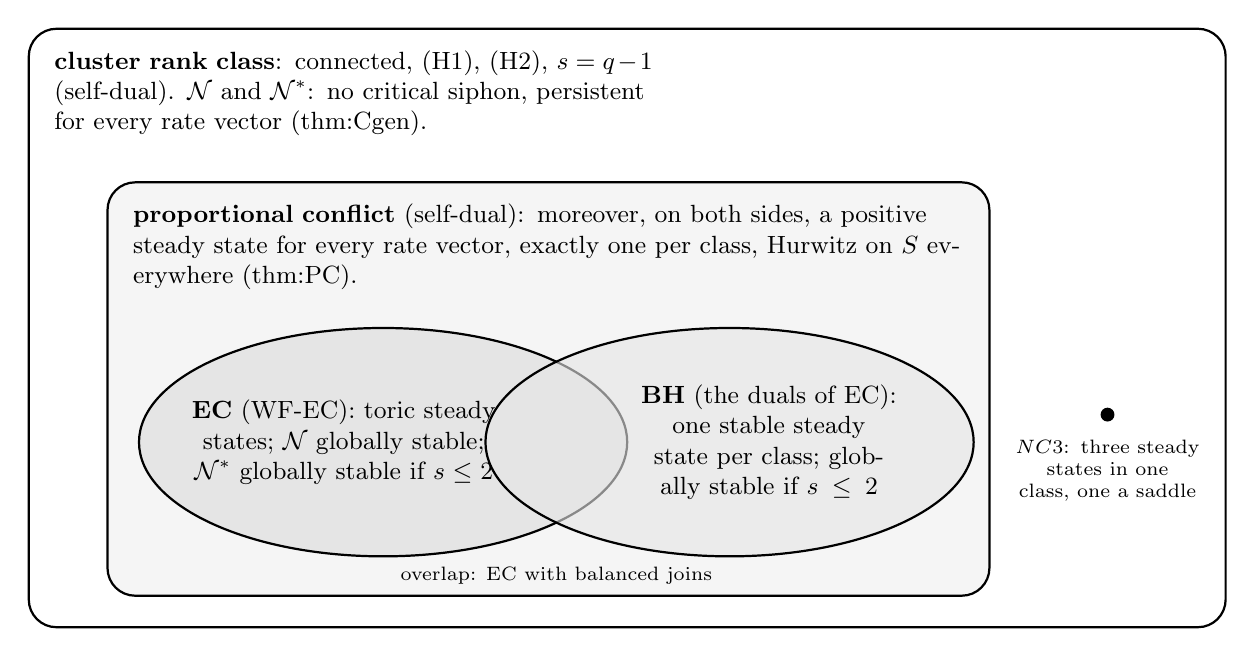
\begin{tikzpicture}[x=1cm,y=1cm,font=\small]
\draw[rounded corners=10pt,thick] (-7.6,-3.9) rectangle (7.6,3.7);
\node[align=left,anchor=north west,text width=7.6cm] at (-7.4,3.55)
 {\textbf{cluster rank class}: connected, (H1), (H2), \(s=q-1\) (self-dual).
  \(\Net\) and \(\Nd\): no critical siphon, persistent for every rate vector (\zcref{thm:Cgen}).};
\draw[rounded corners=10pt,thick,fill=black!4] (-6.6,-3.5) rectangle (4.6,1.75);
\node[align=left,anchor=north west,text width=10.8cm] at (-6.4,1.6)
 {\textbf{proportional conflict} (self-dual): moreover, on both sides, a positive steady state for every rate vector,
  exactly one per class, Hurwitz on \(S\) everywhere (\zcref{thm:PC}).};
\draw[thick,fill=black!10] (-3.1,-1.55) ellipse (3.1cm and 1.45cm);
\draw[thick,fill=black!10,fill opacity=0.6] (1.3,-1.55) ellipse (3.1cm and 1.45cm);
\node[align=center,text width=3.9cm] at (-3.6,-1.55)
 {\textbf{EC} (WF-EC): toric steady states; \(\Net\) globally stable; \(\Nd\) globally stable if \(s\le2\)};
\node[align=center,text width=3.9cm] at (1.8,-1.55)
 {\textbf{BH} (the duals of EC): one stable steady state per class; globally stable if \(s\le2\)};
\node[font=\scriptsize,align=center] at (-0.9,-3.25) {overlap: EC with balanced joins};
\fill (6.1,-1.2) circle (2.5pt);
\node[align=center,text width=2.5cm,font=\scriptsize,anchor=north] at (6.1,-1.4)
 {\(NC3\): three steady states in one class, one a saddle};
\end{tikzpicture}}
\caption{The classes on which the duality transfers structure (all with connectedness, (H1) and (H2)). Each class
inherits the statements of the classes containing it. Global stability of \(\Nd\) for \(s\ge3\) with unbalanced joins, and of general PC
networks, is open. \(NC3\) satisfies the cluster rank equation but not proportional conflict. The networks of \zcref{tab:failures} (\(U\), \(3A\rightleftarrows2A+B\), \(NM\), \(NB\), \(NT\)) violate the cluster rank equation and lie outside the outer class.}\label{fig:classes}
\end{figure}

\subsection{Weakly reversible networks have absolutely consistent duals}

\begin{theorem}[agents E2 and A2]\label{thm:WRdual}
Let \(\Net\) be conservative with \(\im\Gamma\subseteq\im\Ye\) (e.g.\ every product complex in the span of the sources;
in particular \(\Net\) weakly reversible). Then for every \(\kappa\in\Rp^n\), \(\Nd\) has a positive steady state.
Moreover its positive steady-state set is a smooth manifold of dimension \(r-s\), a global graph over a fixed linear
space in logarithmic coordinates.
\end{theorem}
\begin{proof}
Existence (E2, Corollary E2.5\('\)): \(c\tp\Ye=0\) implies \(c\tp\Yp=0\), so \(\ker\Ye\tp\subseteq\ker\Gamma\tp\);
Birch's theorem~\autocite{HornJackson1972,Feinberg2019} applied to \(\Nd\) gives, for every \(\kappa\), a positive \(v\) with
\(v-v^0\in\ker\Ye\tp\) and \(\log v-\log\kappa\in\im\Ye\), which is a steady-state flux. Manifold (A2): factor
\(\im\Gamma=\im\Pi\) with \(\Pi=\Ye R\); in coordinates \(z=q+Rt\), the strictly convex coercive function
\(F_q(t)=\sum_i\kappa_ie^{(\Ye q)_i}e^{\pi_i\cdot t}\) has a unique minimiser, which depends smoothly on \(q\), and its
critical-point equation is the steady-state equation. Details: agent A2's notes (Theorems E, E+), re-derived by V3
(§6).
\end{proof}

The theorem says nothing about classes: \zcref{thm:AF} with \(R=2\) gives weakly reversible \(\Net\) whose dual loses
a species for every rate vector. The convex argument is the classical Birch/moment-map structure (cf.\ Müller and
Regensburger~\autocite{MullerRegensburger2012}).

\section{What the duality does not transfer}\label{sec:nontransfer}

\subsection{Weak reversibility, deficiency, endotacticity, the siphon criterion}

\begin{proposition}[agents G, E]\label{prop:nonWR}
The dual of a weakly reversible network need not be weakly reversible: \(W\) is weakly reversible with deficiency
zero and \(W^*\) is not; the smallest conservative example in agent E's exhaustive families is \(2X_2\rightleftarrows X_1\), with dual
\(K_2\to K_1,\ 2K_1\to2K_2\). If \(\Net\) is weakly reversible with (H3), the rows of \(\Ye\) are pairwise distinct and so are the rows of
\(\Yp\), and \(\Nd\) is weakly reversible iff there is a permutation \(\pi\) of the species with
\((\Yp)_{i\cdot}=(\Ye)_{\pi(i)\cdot}\) for all \(i\); then the deficiency of \(\Nd\) is \((n-s)-c(\pi)\), where \(c(\pi)\) is
the number of cycles of \(\pi\), and \(\mathbf 1_C\) is a conservation law of \(\Net\) for every cycle \(C\) of \(\pi\).
\end{proposition}
\begin{proof}
If \(\Net\) is weakly reversible, every product complex is a source complex, so equal rows of \(\Ye\) would give equal
rows of \(\Yp\) and of \(\Gamma\), excluded by (H3); the reversed network gives the same for \(\Yp\). So \(\Nd\) has \(n\)
distinct sources and \(n\) distinct products. If \(\Nd\) is weakly reversible, each product is a source, which defines
an injective map \(\pi\) with \((\Yp)_{i\cdot}=(\Ye)_{\pi(i)\cdot}\); conversely the complex graph \(i\mapsto\pi(i)\) of a
permutation is a disjoint union of cycles. It has \(n\) complexes and \(c(\pi)\) linkage classes, so the deficiency of
\(\Nd\) is \(n-c(\pi)-s\), and \(\sum_{i\in C}\Gamma_{i\cdot}=\sum_{i\in C}((\Ye)_{\pi(i)\cdot}-(\Ye)_{i\cdot})=0\) for
every cycle \(C\) of \(\pi\). The examples are certified (agent G, Prop.~2.2; V3 §1).
\end{proof}

Blanchini and Giordano already observe that the dual of a reversible network is not even weakly reversible and that
mass action is not preserved~\autocite[p.~493]{BlanchiniGiordano2022}. On the 82\,377 weakly reversible networks with
(H1)--(H3) of agent E's exhaustive families and two seeded samples, the dual is weakly reversible for 98, deficiency
zero is preserved for 43 of 46\,709, the dual is endotactic for 122 of 84\,103 tests and strongly endotactic for 43 of
70\,185 (counted per run, about 1\,700 networks twice; checked by computation, \texttt{gac-duality/computation/notes.md}
§5). So the endotactic persistence theorems
\autocite{CraciunNazarovPantea2013,GopalkrishnanMillerShiu2014} almost never apply to \(\Nd\).

\begin{proposition}[the siphon criterion is not self-dual; agent G]\label{prop:ADLS}
\(H\colon 2A\rightleftarrows2B,\ 2A\rightleftarrows A+B\) is weakly reversible with (H1)--(H3), and its only minimal
siphon \(\{A,B\}\) supports \(a+b\). Its dual \(2U_1+2U_3+U_4\to2U_2+U_3+2U_4,\ 2U_2+U_4\to2U_1+U_3\) satisfies
(H1)--(H3) and has the critical siphon \(\{U_4\}\).
\end{proposition}
\begin{proof}
Checked in exact arithmetic (\texttt{certify\_duality.py}, claim ``S5 H''); agent G, re-checked by V3.
\end{proof}

The converse also fails (agent E: \(X_4\rightleftarrows X_2+X_3,\ 2X_4\rightleftarrows X_1+X_3\)); among the 82\,377
networks the criterion holds for \(\Net\) but not \(\Nd\) in 5\,252 cases and conversely in 924 (checked by
computation). In intermediate dimensions almost every weakly reversible network has a critical siphon (agent E), so
the criterion rarely applies on either side.

\subsection{Persistence}

\begin{example}[agent G; strengthened by agent E]\label{ex:M}
\(M\colon 3A\rightleftarrows2A+B\) is reversible with one linkage class and deficiency zero, and
\(\dot a=a^2(k_2b-k_1a)\): every class converges to its unique positive equilibrium. Its dual
\(M^*\colon 3U+2V\to2U+3V,\ V\to U\) (\(U=K_1\), \(V=K_2\) in \zcref{fig:revdual}) has \(\dot v=v(\kappa_1u^3v-\kappa_2)\), so on a class \(u+v=T\),
\(\dot v\le-(\kappa_2/2)v\) whenever \(v\le\min(T,\kappa_2/(2\kappa_1T^3))\): \(M^*\) is non-persistent for every rate
vector and in every class. With unit rates and \(T=2\) the class contains the two positive equilibria \(v=1\) and a root
of \(v^3-5v^2+7v-1\) in \((1/8,1/2)\), and \(v\to0\) from \((15/8,1/8)\) since \(h(v)=(2-v)^3v\) is increasing on
\([0,1/8]\) with \(h(1/8)=3375/4096\), so \(\dot v\le-(721/4096)v\). Both networks have \(\Gamma=\bigl(\begin{smallmatrix}-1&1\\1&-1\end{smallmatrix}\bigr)\)
and satisfy (H1)--(H3).
\end{example}

The smallest instance (V3) is \(X\colon 2X_2\rightleftarrows X_1+X_2\), whose dual \(K_2\to K_1,\ 2K_1+K_2\to
K_1+2K_2\) satisfies \(\dot K_2=K_2(\kappa_2K_1^2-\kappa_1)\) and loses \(K_2\) in every class with \(\kappa_2T^2<\kappa_1\),
for every rate vector (\zcref{ex:S1}). The mechanism of \zcref{ex:M} is general.

\begin{proposition}[drain species; agent E]\label{prop:drain}
Let \(\mathcal X\) be conservative and \(i\) a species such that (a) some reaction has source exactly \(d_0X_i\) and
consumes \(X_i\), and (b) every reaction with a net production of \(X_i\) (\(\Gamma_{ij}>0\)) has a source with
\(X_i\)-coefficient \(>d_0\). Then for every
rate vector and every class, every positive solution with \(x_i(0)\) small has \(x_i(t)\to0\).
\end{proposition}
\begin{proof}
On a class all coordinates are bounded by some \(T\); the terms of \(\dot x_i\) with \(\Gamma_{ij}>0\) are \(\le Cx_i^{d_0+1}\) and the
draining reaction contributes \(-c_0x_i^{d_0}\), so \(\dot x_i\le x_i^{d_0}(Cx_i-c_0)\).
\end{proof}

Hypothesis (b) never holds on a weakly reversible network itself (the cycle through the source \(d_0e_i\) must raise
the coefficient of \(X_i\) to \(d_0\); V3), so every drain species of \(\Nd\) is an asymmetry of the duality.

\begin{theorem}[drain sets; agent Q1]\label{thm:drainsets}
Let \(\mathcal X\) be conservative and \(Z\) a set of species with weights \(w\in\Rp^Z\) and degrees \(d\in\mathbb{Z}^Z_{\ge1}\)
such that, with \(V=\langle w,x_Z\rangle\): (D1) for each \(i\in Z\) some reaction has source exactly \(d_iX_i\) and
strictly decreases \(V\); (D2) every reaction that strictly increases \(V\) has a source \(y\) with
\(\sum_{i\in Z}y_i/d_i>1\). Then for every rate vector and every class there is \(\delta>0\) such that every solution
with \(V(x(0))<\delta\) has \(x_Z(t)\to0\). \(Z\) contains no support of a nonnegative conservation law.
\end{theorem}
\begin{proof}
With \(u_i=x_i^{d_i}\), \(U=\max u_i\) and \(\theta=\sum_i\beta_i/d_i>1\) for a source \(\beta\) of (D2),
\(x_Z^\beta\le U^\theta\le U^{\theta-1}\sum_iu_i\), and \(U^{\theta-1}\to0\) as \(V\to0\). So for small \(V\),
\(\dot V\le-(c/2)\sum_ix_i^{d_i}\), and \(V\to0\).
\end{proof}

\begin{example}[agents E, E2, Q1]\label{ex:drain}
(1) \(X_4\to3X_3\to X_1+2X_2\to3X_2\to X_4\) is weakly reversible with deficiency zero, \(s=3\), one linkage class and
(H1)--(H3), hence globally stable (Anderson~\autocite{Anderson2011}; Pantea~\autocite{Pantea2012}); its dual satisfies
(H1)--(H3) and the species dual to \(X_1+2X_2\to3X_2\) is a drain species. (2) The 5-cycle
\(X_5\to3X_4\to X_2+X_4\to X_1+2X_3\to3X_3\to X_5\) (\(s=4\), deficiency zero) has a dual with the drain species
dual to \(X_1+2X_3\to3X_3\). (3) For \(C\colon 2X_3\to X_2+X_3\to X_1+X_3\to2X_3\) (\(s=2\), deficiency zero), the
dual \(K_3\to K_2,\ K_2\to K_1,\ 2K_1+K_2+K_3\to K_1+K_2+2K_3\) has \(V=K_2+2K_3\) with
\(\dot V=-\kappa_1K_3-\kappa_2K_2+2\kappa_3K_1^2K_2K_3\): \(\{K_2,K_3\}\) is a drain set and there is no drain species.
(4) Weak reversibility and purity together do not help: \(X_4\rightleftarrows X_2+X_3,\ 3X_3\rightleftarrows X_1+2X_4\)
is pure and weakly reversible with (H1)--(H3), and its dual has a drain set of two species (E2; this refutes a
conjecture of Q1).
\end{example}

Counts (checked by computation): among the 82\,377 weakly reversible networks with (H1)--(H3) of agent E's
families of molecularity at most three (all with \(n\le6\)), 141 have a dual with a drain species, all with \(s\le2\);
in E's exhaustive molecularity-three families with four and five species, 103 duals with \(s=3\) have one; in E2's
seeded molecularity-three samples with \(s=4\), 238 (\texttt{gac-duality/computation/notes.md} §5,
\texttt{gac-duality/round2/computation/notes.md} §3). Drain sets with \(|Z|\le4\) occur for 1\,735 duals of E's weakly
reversible networks with (H1)--(H3), 1\,432 of them without a drain species (Q1,
\texttt{gac-duality/round2/persistence/notes.md} §3); over all of E's records, 199 duals with \(s=2\) have a drain
species, a count recounted by V3.

\subsection{Convergence}

Persistence of the dual for all rates does not give convergence, even with a unique equilibrium in every class.

\begin{theorem}[agent A2]\label{thm:O}
Let \(\Net\) be the 3-cycle \(3X_3\to X_1+X_2\to X_2+2X_3+3X_4\to3X_3\) (weakly reversible, deficiency zero, \(s=2\),
(H1)--(H3)). Write \(a,b,c\) for the dual species and \(\alpha,\beta,\gamma,\delta\) for the dual rates, so that
\(\Nd\colon b\to a,\ b+c\to a+b,\ 3a+2c\to2b+3c,\ 3c\to3b\). Then for every rate vector \(\Nd\) is persistent
(\zcref{thm:A}) and has exactly one positive equilibrium in each class \(a+b+c=T\). At
\((\alpha,\beta,\gamma,\delta)=(17,400,70000,10^6)\) and \(T=201/100\) the equilibrium is \((1,1,1/100)\), a hyperbolic
source, and the class contains a nonconstant periodic orbit.
\end{theorem}
\begin{proof}
Uniqueness: \(\dot b-2\dot c=(2\beta c-\alpha)b+9\delta c^3\), so equilibria have \(0<c<\alpha/(2\beta)\),
\(b=9\delta c^3/(\alpha-2\beta c)\) and \(a^3=3\delta c(\alpha+\beta c)/(\gamma(\alpha-2\beta c))\); both are
increasing in \(c\) (numerators \(c^2(3\alpha-4\beta c)\) and \(\alpha^2+2\alpha\beta c-2\beta^2c^2\)), so \(a+b+c\)
increases from \(0\) to \(\infty\). At the given rates the fluxes at \((1,1,1/100)\) are \((17,4,7,1)\), and the Jacobian
in \((b,c)\) is \(J=\bigl(\begin{smallmatrix}-59&3658\\-25&79\end{smallmatrix}\bigr)\), trace \(20\), determinant
\(86\,789\), eigenvalues \(10\pm i\sqrt{86\,689}\). With \(H=\bigl(\begin{smallmatrix}93\,655&-290\,457\\-290\,457&
13\,471\,234\end{smallmatrix}\bigr)\), positive definite, \(J\tp H+HJ=3\,471\,560\,I\), so the equilibrium is a
repeller and lies in the \(\omega\)-limit set of no other point. By \zcref{thm:A} every \(\omega\)-limit set of an
interior point is a compact subset of the open triangle, and it contains no equilibrium; Poincaré--Bendixson gives a
periodic orbit.
\end{proof}

\begin{figure}[ht]
\centering
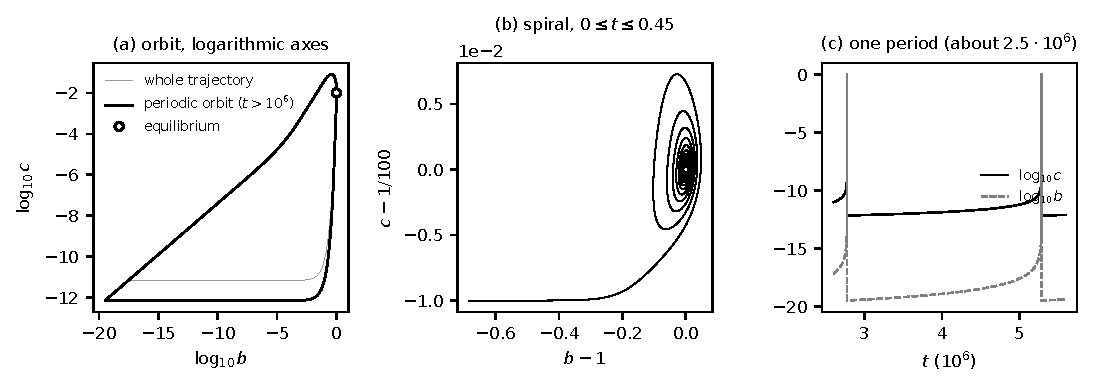
\includegraphics[width=\linewidth]{figures/theoremO-orbit.pdf}
\caption{Numerical illustration of \zcref{thm:O}, not part of the proof. (a) The trajectory from
\((1,1-10^{-4},10^{-2}+10^{-4})\) in logarithmic coordinates, and its late part, which traces the periodic orbit.
(b) The spiral leaving the source. (c) One period of the orbit, about \(2.51\cdot10^6\) time units, during which
\(c\) drops to about \(7\cdot10^{-13}\) and \(b\) to about \(3\cdot10^{-20}\), near the vertex \((T,0,0)\). Integrated
in the variables \(\log a,\log b,\log c\) with a stiff implicit solver (\texttt{scripts/figures.py}); in linear
coordinates the solver wrongly appears to converge to the vertex (V3).}\label{fig:orbitO}
\end{figure}

V3 adds two remarks. The orbit is persistent but passes within about \(10^{-12}\) of the boundary, so naive numerical
integration in linear coordinates wrongly suggests extinction: numerical persistence tests on these duals need
logarithmic coordinates. And \zcref{thm:O} does not contradict Blanchini and Giordano~\autocite{BlanchiniGiordano2022}:
their Theorem~1 transfers \emph{structural} local stability (for all admissible derivative matrices) under their
Assumption~3 (a rate depends on \(x_i\) iff \(\Gamma_{ij}<0\)), which both \(\Net\) (\(X_2\) is a catalyst in
\(X_1+X_2\to X_2+2X_3+3X_4\)) and \(\Nd\) (\(b\) is a catalyst in \(b+c\to a+b\)) violate.

\section{Persistence of duals in low rank}\label{sec:lowrank}

\subsection{Rank one: an exact test and a dichotomy}

Let \(\mathcal M\) be a conservative network of rank one with reaction vectors \(c_jg\), \(g\in\mathbb{Z}^p\) primitive, so
that \(g\) has entries of both signs. A positive class is a segment \(x_0+\xi g\), and \(\dot\xi=F(\xi)=\sum_jc_j\kappa_jx^{y_j}\).
Put \(N_-=\{i:g_i<0\}\) and \(N_+=\{i:g_i>0\}\). An \emph{upper face} is a nonempty \(Z\subseteq N_-\) (\(\sigma=+1\)), a
\emph{lower face} a nonempty \(Z\subseteq N_+\) (\(\sigma=-1\)); every such \(Z\) is the zero set of an endpoint of some
class. For a face, let \(o_Z(j)=\sum_{i\in Z}(y_j)_i\) over the reactions with \(c_j\ne0\), \(\mu\) its minimum and \(J\) the
minimisers; \(j\in J\) is \emph{inward} if \(\sigma c_j<0\) and \emph{outward} otherwise; \(\beta_j\) is \(y_j\) restricted to
the species outside \(Z\). The face is IN if all of \(J\) is inward, OUT if all is outward, ESC if some outward
\(\beta_j\) lies outside the convex hull of the inward ones, and DOM otherwise (\zcref{fig:faces}).

\begin{figure}[ht]
\centering
\begin{tikzpicture}[x=1cm,y=1cm,font=\small,
  arr/.style={-{Stealth[length=2mm]},thick}]
\foreach \k/\name/\txt in {0/IN/{lowest-order terms all inward: the endpoint repels, for every \(\kappa\) and every class},
  1/OUT/{all outward: the endpoint attracts, for every \(\kappa\), in every class reaching this face},
  2/ESC/{mixed; some outward exponent lies outside the inward hull: for every \(\kappa\) some class is attracted},
  3/DOM/{mixed; every outward exponent lies in the inward hull: the outcome depends on \(\kappa\)}} {
  \begin{scope}[yshift=-\k*1.45cm]
  \draw[thick] (0,0) -- (3.2,0);
  \fill (3.2,0) circle (2.2pt);
  \node[font=\scriptsize,anchor=west] at (3.3,0) {\(Z\)};
  \node[font=\bfseries\small,anchor=east] at (-0.2,0) {\name};
  \node[anchor=west,text width=8.2cm,font=\scriptsize] at (4.3,0) {\txt};
  \end{scope}}
\draw[arr] (3.0,0.25) -- (1.9,0.25);
\draw[arr] (1.9,-1.2) -- (3.0,-1.2);
\draw[arr] (3.0,-2.65) -- (1.9,-2.65);
\draw[arr] (1.9,-3.15) -- (3.0,-3.15);
\node[font=\scriptsize,anchor=east] at (1.85,-3.15) {at \(e^{tw}\)};
\draw[arr] (3.0,-4.1) -- (1.9,-4.1);
\draw[arr,dashed] (1.9,-4.6) -- (2.8,-4.6);
\node[font=\scriptsize,anchor=east] at (1.85,-4.6) {AM--GM};
\end{tikzpicture}
\caption{The four face types of the rank-one test (\zcref{thm:S1}). Each line is a compatibility class (a segment)
ending at a boundary point whose zero set is the face \(Z\); arrows show the lowest-order terms of the flow near that
point (left: towards the interior; right: towards the face). For ESC, a separating direction \(w\) makes an outward
term win at boundary points \(\exp(tw)\) for large \(t\); for DOM, every outward exponent lies in the convex hull of the
inward ones, so weighted AM--GM bounds it when the outward rate constants are small.}\label{fig:faces}
\end{figure}

\begin{lemma}[endpoint expansion; agent Q1]\label{lem:endpoint}
At an upper endpoint \(x^+\) with zero set \(Z\), along \(x^+-\varepsilon g\),
\[F=\varepsilon^\mu L(\kappa,x^+)+O(\varepsilon^{\mu+1}),\qquad L=\sum_{j\in J}c_j\kappa_j\prod_{i\in Z}|g_i|^{(y_j)_i}
\prod_{i\notin Z}(x^+_i)^{(y_j)_i};\]
similarly at lower endpoints. \(\mathcal M\) is persistent for a given \(\kappa\) iff no
endpoint of any class attracts nearby points of its class.
\end{lemma}
\begin{proof}
Agent Q1's notes, Lemmas 1.1--1.2 (along a class \(F\) is a polynomial in \(\varepsilon\), and the dynamics on a segment
is one-dimensional); re-derived by V3 (§3).
\end{proof}

\begin{theorem}[rank one; agent Q1, with V3's wording of (4)]\label{thm:S1}
Let \(\mathcal M\) be conservative of rank one.
\begin{enumerate}
\item \(\mathcal M\) is persistent for every rate vector iff every face is IN.
\item If some face is OUT or ESC, \(\mathcal M\) is non-persistent for every rate vector.
\item If every face is IN or DOM, some face is DOM, and all DOM faces lie at the same end, the set of rate vectors for
which \(\mathcal M\) is persistent contains a nonempty open set, and so does its complement.
\item If DOM faces occur at both ends, the set of rate vectors for which \(\mathcal M\) is persistent is semialgebraic; it
can be a hypersurface.
\end{enumerate}
\end{theorem}
\begin{proof}
(1) If all faces are IN, \(\sigma L<0\) always. Otherwise take \(\kappa_{j_0}\) large for an outward \(j_0\) at
\(x^+=(0\text{ on }Z,1\text{ off }Z)\). (2) OUT: \(\sigma L>0\) always. ESC: a vector \(w\) separating an outward \(\beta_0\)
from the inward hull; at \(x^+=\exp(tw)\) off \(Z\) the outward term dominates as \(t\to\infty\). (3) Weighted AM--GM
bounds each outward monomial by the inward ones; small outward rate constants make \(\sigma L<0\) everywhere, by
finitely many strict linear inequalities in \(\kappa\). (4) The condition is a first-order formula in \(\kappa\)
(Tarski--Seidenberg); example \(B\) below.
\end{proof}

For a rank-one network \(\Net\) with reaction vectors \(b_ja\), \(\Gamma(\Nd)=ba\tp\): a face of \(\Nd\) is a nonempty set
\(Z\) of reactions of \(\Net\) all oriented the same way along \(a\), the order of \(\rho_i\) is the \emph{load}
\(\ell_Z(i)=\sum_{j\in Z}(y_j)_i\), and \(\rho_i\) is inward iff \(X_i\) is a net product of \(Z\).

\begin{corollary}[the test on \(\Net\); agent Q1]\label{cor:S1N}
For \(\Net\) of rank one with (H2), \(\Nd\) is persistent for every rate vector iff for every nonempty set \(Z\) of reactions
with a common orientation, every species with \(a_i\ne0\) minimising \(\ell_Z\) is a net product of \(Z\).
\end{corollary}
\begin{proof}
\zcref{thm:S1}(1) for \(\mathcal M=\Nd\), which is conservative by (H2), with the dictionary above.
\end{proof}

\begin{theorem}[all-or-none in rank one; agent Q1]\label{thm:S1WR}
Let \(\Net\) have rank one and suppose that in every linkage class the two complexes extreme along \(a\) are sources
(e.g.\ \(\Net\) weakly reversible). Then \(\Nd\) has no DOM face, so it is persistent for every rate vector or for none.
\end{theorem}
\begin{proof}
A linkage class lies on a line \(y_L+ta\). Suppose a forward face \(Z\) is DOM, with outward species \(o\) and inward
species \(q\) of minimal load, and \(\beta_o=\sum_q\lambda_q\beta_q\). Then \(\phi_o-\phi_v\) (\(v=\sum\lambda_qX_q\)) is affine
in \(t\) with negative slope and vanishes at the sources of reactions outside \(Z\), so at most one position per linkage
class is such a source; the extreme forward position is one, every reaction of \(Z\) leaves a position where
\(\phi_o-\phi_v>0\), and summing over \(Z\) contradicts the equality of the minimal loads.
\end{proof}

\begin{corollary}[agent Q1, with V3's correction]\label{cor:Cpure}
If \(s=1\), \(\Net\) satisfies (H1) and (H2), and no reaction of \(\Net\) has one of its net products in its source (e.g.\
\(\Net\) pure), \(\Nd\) is persistent for every rate vector. (H1) is needed: \(0\rightleftarrows A\) is pure, weakly
reversible and consistent, and its dual \(K_2\to K_1\) loses \(K_2\). If \(n=2\), \(s=1\) and (H1)--(H3) hold, \(\Nd\) is persistent for every
rate vector iff every source contains strictly more of the species its reaction consumes than of the one it produces.
\end{corollary}
\begin{proof}
By (H1) the vector \(a\) has entries of both signs. Let \(Z\) be a face of \(\Nd\) (\zcref{cor:S1N}). A species with
\(a_i\neq0\) is a net reactant of every reaction of \(Z\) or a net product of every reaction of \(Z\). A net reactant
occurs in every source of \(Z\), so its load is at least \(|Z|\ge1\); a net product occurs in no source of \(Z\) by
hypothesis, so its load is \(0\), and net products exist by (H1). So every species of minimal load with \(a_i\neq0\) is a
net product, every face is IN, and \zcref{cor:S1N} applies. If \(n=2\), every reaction consumes one species and
produces the other, the reactions of one orientation all consume the same species, loads add over \(Z\), so the
singleton faces decide, and \(\{j\}\) is IN iff \(y_j\) contains more of the consumed than of the produced species.
\end{proof}

\begin{example}[rank one; agents Q1, E2, V3]\label{ex:S1}
\(X\colon 2X_2\rightleftarrows X_1+X_2\) (reversible, deficiency zero, (H1)--(H3)): the face \(\{K_2\}\) of
\(X^*\) is ESC, so \(X^*\) is NONE although it has no drain species and no drain set; it is the smallest weakly
reversible network with (H1)--(H3) and a NONE dual (V3: one species is impossible, \(X_1\rightleftarrows X_2\) is ALL,
and V3's enumeration of the family \((2,2,4)\) finds \(X\) first). For \(3A\rightleftarrows2A+B\) the face \(\{K_2\}\) is OUT.
\(P\colon 2X_1+X_3\rightleftarrows3X_1+2X_2,\ 2X_2+X_3\rightleftarrows X_1+4X_2\) (weakly reversible, \(s=1\)): every
singleton face of \(P^*\) is IN, but the face formed by the two forward reactions is ESC, so \(P^*\) is NONE.
\(S\colon X_1+X_2\to2X_2+2X_3,\ X_1+X_2+2X_3\to2X_1\) (not weakly reversible): \(\dot K_1=K_2((\kappa_2-\kappa_1)K_1+2\kappa_3K_2)\)
for \(S^*\colon K_1+K_2\to2K_2,\ K_1+K_2\to2K_1,\ 2K_2\to2K_1\), persistent exactly for \(\kappa_1>\kappa_2\) (DOM at one end).
\(B\colon X_1+X_2\to2X_2,\ X_1+X_2\to2X_1\): \(\dot K_1=(\kappa_2-\kappa_1)K_1K_2\), persistent only on \(\kappa_1=\kappa_2\) (DOM at both
ends). In rank two the corollary for pure networks fails, already without weak reversibility:
\(Q\colon X_1\to X_2,\ X_1\to X_3,\ X_2+X_3\to2X_1\) has \((K_2-K_1)^\cdot=(\kappa_3-\kappa_2)K_3\), so \(Q^*\) is
non-persistent for every rate vector with \(\kappa_2\neq\kappa_3\) (the hypersurface \(\kappa_2=\kappa_3\) was not
analysed); \zcref{ex:drain}(4) shows that it also fails for weakly reversible pure networks.
\end{example}

\paragraph{Counts and credits.} On eight exhaustive families of weakly reversible rank-one networks with (H1)--(H3)
(up to 3\,544 networks per family), \(\Nd\) is persistent for every rate vector for 11--33\,\% of the networks of each
family with more than one member (381 of 3\,544 to 4 of 12; the family \((4,3,4)\) has a single network, which is ALL)
and for none for the rest, never SOME (Q1; recounted by V3 with its own generator, identical numbers). E2's separate
decision procedure agrees on
all 4\,754 rank-one networks with (H1), (H2) of E's records. The face test restricts the parallel-sweep test of
Craciun, Nazarov and Pantea~\autocite{CraciunNazarovPantea2013} and Pantea~\autocite{Pantea2012} to the directions
\(\mathbf 1_Z\). Zhang, Gao and Dochain~\autocite[Thm~3.10]{ZhangGaoDochain2023} prove persistence of one-dimensional
\(W_I\)-endotactic networks for all rates, which implies the ``if'' half of \zcref{thm:S1}(1) under a stronger
hypothesis: V3's network \(A+B\to2A,\ 2A\to A+B,\ 3A+B\to4A\) has every face IN (\(\dot a=a(k_1b-k_2a+k_3a^2b)\)) but is not
\(W_I\)-endotactic. The converse halves, the DOM case and the dichotomy were not found.

\subsection{Weak reversibility excludes dominated facets in every rank}

\begin{theorem}[agent D2, in V3's general form]\label{thm:W}
Let \(Z\) be a set of reactions of \(\Net\) with positively parallel reaction vectors \(b_ja\) (a facet set of \(\Nd\), in any
rank), and suppose every product of a reaction of \(Z\) is a source complex (e.g.\ \(\Net\) weakly reversible). Then the facet
\(Z\) of \(\Nd\) is not DOM: there are no outward species \(o\) and inward species \(q\) of minimal load with
\((y_l)_o=\sum_q\lambda_q(y_l)_q\) for every \(l\notin Z\), with \(\lambda_q\ge0\) and
\(\sum_q\lambda_q=1\).
\end{theorem}
\begin{proof}
\(\phi(y)=y_o-\sum_q\lambda_qy_q\) vanishes on the sources outside \(Z\) and drops along each reaction of \(Z\). A source of
\(Z\) with \(\phi\le0\) would start an infinite chain of distinct complexes with strictly decreasing \(\phi\). So \(\phi>0\) on
the sources of \(Z\), contradicting \(\sum_{j\in Z}\phi(y_j)=\mu-\mu=0\).
\end{proof}

\subsection{Rank two}\label{sec:rank2}

Let \(s=2\) and let \(\Net\) satisfy (H1)--(H3), so that the positive classes of \(\Nd\) are compact convex polygons.
Factor \(\Gamma=\Pi\hat G\); the class of \(K^0\) is the polygon \(\{X\in\mathbb{R}^2:K^0_j+\langle g_j,X\rangle\ge0\}\),
whose edges have inward normals among the reaction vectors \(g_j\) of \(\Net\). Every point with zero set exactly a facet
set lies in the relative interior of an edge of some class, and every point with zero set a vertex set is a vertex of
some class (agent D2, Lemma~2.1). On an open edge whose zero set \(Z\) is a siphon of \(\Nd\) (a \emph{siphon edge};
its facet set is a \emph{siphon facet}) only the reactions of \(\Nd\) whose source avoids \(Z\) act, and they move
along the edge; their sum is the \emph{edge flow}, \emph{one-way} if all its terms have one sign, \emph{two-way} if both
signs occur, \emph{zero} if there is no such reaction. The finer notions used in \zcref{prop:none-cert}
(two-coloured edge flows, the transverse order \(\mu\), tropically Hurwitz vertices, centre manifolds, attracting
linear functions and sectors) are defined in agent D2's notes (\texttt{gac-duality/round3/dichotomy/notes.md} §2--3).

\begin{lemma}[agent D2]\label{lem:A}
If \(p\) is a boundary point of the \(\omega\)-limit set \(\Omega\) of an interior point, then \(p\) is an equilibrium or lies
in an open edge whose zero set is a siphon of \(\Nd\), the field is tangent to the edge there, and the whole orbit of \(p\)
stays in the open edge. Every vertex in \(\Omega\) is an equilibrium.
\end{lemma}
\begin{proof}
Agent D2's notes, Lemma A (the siphon edge is invariant in both time directions for the polynomial field); re-derived by
V3 (§5).
\end{proof}

\begin{theorem}[persistence certificate; agent D2, corrected by V3]\label{thm:P2}
Suppose that for every rate vector and every class: (A1) every siphon facet has a one-way edge flow, or is IN with a
two-way edge flow that cannot vanish identically; (A2) every vertex equilibrium \(e\) has a neighbourhood \(U_e\) and a
\(C^1\) function \(V_e\ge0\) with \(V_e(e)=0\), \(V_e>0\) on the interior and \(\dot V_e>0\) on \(U_e\cap\operatorname{int}P\);
(A3) some edge is not a siphon edge. Then \(\Nd\) is persistent for every rate vector.
\end{theorem}
\begin{proof}[sketch]
A boundary point of \(\Omega\) leads (\zcref{lem:A}) to a boundary equilibrium \(e\in\Omega\), which repels the interior by
(A2) or by the normal coordinate of an IN edge, and is isolated: along an interior total orbit in a compact invariant
set near \(e\), \(V_e\) is strictly increasing, so its \(\alpha\)- and \(\omega\)-limit sets lie in \(\partial P\); near \(e\)
the only invariant subset of \(\partial P\) is \(\{e\}\) (boundary orbits are monotone along the edges), so both limit
sets are \(\{e\}\), which contradicts the strict increase of \(V_e\) between them since \(V_e(e)=0\) (V3's addition).
The Butler--McGehee lemma~\autocite[Thm~4.1]{ButlerWaltman1986} gives a point of \(\Omega\setminus\{e\}\) converging to \(e\),
necessarily on a siphon edge flowing into \(e\); repeating upstream around the boundary circle makes every edge a siphon
edge, contradicting (A3). This is a planar version of the acyclicity theorem of Butler and
Waltman~\autocite{ButlerWaltman1986} and Hale and Waltman~\autocite{HaleWaltman1989}, with \zcref{lem:A} replacing their
invariant-boundary hypothesis. Full proof in agent D2's notes, re-derived by V3.
\end{proof}

\begin{proposition}[extinction certificates; agent D2, with V3's repair]\label{prop:none-cert}
Each of the following gives, for every rate vector, a class with an interior trajectory converging to the boundary:
(E) an OUT or ESC siphon facet whose edge flow is two-coloured with minimal transverse order \(\mu=1\), or zero with
\(\mu=1\) (an edge equilibrium with an attracting normal eigenvalue, whose stable manifold enters the interior; V3 repaired
the written proof for \(\mu=1\), which covers every use); (H) a tropically Hurwitz vertex; (CM) an attracting centre
manifold at a vertex; (L) an attracting linear function; (S) an attracting sector; (B) a product of two rank-one blocks,
one of them NONE.
\end{proposition}
\begin{proof}[sketch]
Proofs in agent D2's notes (Propositions E, H, CM, L, S, B; \zcref{tab:concordance}). (E) for
\(\mu=1\), as repaired by V3: on the facet there is a point \(p^*\) with zero set \(Z\), zero edge flow and normal
coefficient \(L(p^*)<0\); it is an equilibrium of its class, and the stable manifold of the eigenvalue \(L(p^*)\) is
transverse to the invariant edge and enters the interior. (H): Cauchy--Binet for a sum of rank-one \(2\times2\)
matrices; a Hurwitz vertex attracts an open set of its class. (B): the two blocks decouple. (CM), (L), (S) are standard
centre-manifold, Lyapunov and sector arguments, written as sketches in D2's notes and checked by V3 at sketch level and
on the worked examples below.
\end{proof}

Examples (certified identities): for \(2X_3\to X_2\to2X_1+X_3\to2X_3\) the dual \(2K_3\to2K_2,\ K_2\to K_1,\
2K_1+K_3\to K_2+2K_3\) has \(\dot K_3=K_3(\kappa_3K_1^2-2\kappa_1K_3)\), the only siphon edge is \(\{K_3\}\) (IN) and the only
siphon vertex \(\{K_2,K_3\}\): ALL. For \(2X_3\to2X_2+X_3\to X_1+X_2+X_3\to2X_3\) the facet \(\{K_3\}\) is ESC with zero edge
flow and \(\mu=1\): NONE by (E). For \(2X_3\to X_2+X_3\to X_1+X_2\to2X_3\), at \((0,T,0)\) the reduced equation on the centre
manifold has the coefficient \(\kappa_3T(\kappa_2T-\kappa_1)/(\kappa_1+\kappa_2T)\): NONE by (CM). For
\(2X_3\to2X_2+X_3\to2X_1+X_3\to2X_3\), \(V=K_2+2K_3\) has \(\dot V=-2\kappa_1K_3^2-2\kappa_2K_2^2+2\kappa_3K_1^2K_2K_3\), negative
definite near \((T,0,0)\) when \(\kappa_3^2T^4<4\kappa_1\kappa_2\): NONE by (L). For \(2X_3\to X_2\to X_1+X_3\to2X_3\) the
vertex \((T,0,0)\) of the dual has the linearisation \(\bigl(\begin{smallmatrix}-\kappa_2&\kappa_1+\kappa_3T^2\\0&\kappa_3T^2-
\kappa_1\end{smallmatrix}\bigr)\), Hurwitz when \(\kappa_3T^2<\kappa_1\) (E2's vertex scaling).

\paragraph{Counts (checked by computation).} Among the 18\,861 weakly reversible networks with (H1)--(H3) and
\(s=2\) in
agent E's records, E2 certified 2\,988 ALL (no critical siphon in \(\Nd\)) and 1\,048 NONE (drain species, drain sets,
vertex scaling); D2's certificates decide 14\,654 of the remaining 14\,825: in all, ALL 4\,873, NONE 13\,817, undecided
171, and no network meets an ALL and a NONE certificate (\texttt{gac-duality/round3/dichotomy/notes.md} §4; re-run by
V3, whose own sampled test of the ALL verdicts found no Hurwitz boundary vertex). The undecided ones are mostly
ties in \(\kappa\) at a vertex, as in the next example.

\begin{example}[a vertex tie; agent D2]\label{ex:U}
For \(3X_3\to2X_1+X_2\to X_2+2X_3\to3X_3\), with the reactions numbered \(3X_3\to2X_1+X_2\), \(X_2+2X_3\to3X_3\),
\(2X_1+X_2\to X_2+2X_3\), the dual \(2K_3\to2K_1,\ K_2+K_3\to K_1+K_3,\ 3K_1+2K_2\to3K_2+2K_3\) satisfies,
with \(a=K_2\), \(b=K_3\), \(K=\kappa_3K_1^3\), \(z=a/b\) and \(u=b/a\),
\(\dot z=a[(2\kappa_1-\kappa_2)+Kz(1-2z)]\), \(\dot u=a[(\kappa_2-2\kappa_1)u^2-Ku+2K]\), \(\dot a=a^2(K-\kappa_2u)\) and
\(\dot b=b^2(-2\kappa_1+2Kz^2)\). The sign of \(2\kappa_1-\kappa_2\) at the vertex \((T,0,0)\) cannot be changed by scaling the
class, and the dual is NONE by three different mechanisms for \(\kappa_2>2\kappa_1\), \(<\) and \(=\).
\end{example}

\paragraph{Conjecture F is false.} Q1 and D2 conjectured that a realisable OUT facet forces NONE (D2 proved it for zero
edge flows with \(\mu=1\), and for two-coloured edge flows with \(\mu=1\) with V3's repair). Agent A2 refuted it.

\begin{theorem}[agent A2]\label{thm:A}
The dual of \(3X_3\to X_1+X_2\to X_2+2X_3+3X_4\to3X_3\) (\zcref{thm:O}) is persistent for every rate vector, although
every positive class has the OUT facet \(c=0\).
\end{theorem}
\begin{proof}
\(\Net\) is weakly reversible with deficiency zero, rank two and (H1)--(H3) (law \((11,1,4,1)\), value 12 on every complex;
flux \((1,1,1)\)). The dual field is \(\dot a=\alpha b+\beta bc-3\gamma a^3c^2\), \(\dot b=-\alpha b+2\gamma a^3c^2+3\delta c^3\),
\(\dot c=-\beta bc+\gamma a^3c^2-3\delta c^3\), on the triangles \(a+b+c=T\). On the open edges \(a=0\) and \(b=0\) the
field points strictly inward, at \((0,T,0)\) and \((0,0,T)\) it is nonzero, and on \(c=0\) the orbit \(b(t)=b(0)e^{-\alpha t}\)
leaves the triangle in finite backward time; so \(\Omega\cap\partial P\subseteq\{(T,0,0)\}\). The edge \(c=0\) is OUT: the only
term of order one in \(c\) is \(-\beta bc\). With \(V=c\,e^{-\beta b/\alpha}\),
\begin{equation}\label{eq:A1}
\alpha\,\dot c-\beta c\,\dot b=c^2\bigl[\alpha\gamma a^3-(3\alpha\delta+2\beta\gamma a^3)c-3\beta\delta c^2\bigr],
\end{equation}
so \((\log V)^\cdot=c\,[\gamma a^3-(3\delta+2\beta\gamma a^3/\alpha)c-3\beta\delta c^2/\alpha]\ge c\,(\gamma T^3/8-E\varepsilon)
\ge c\,\gamma T^3/16>0\) at the interior points of \(\{b+c<\varepsilon\}\), with
\(E=3\delta+2\beta\gamma T^3/\alpha+3\beta\delta/\alpha\), \(\varepsilon=\min(T/2,1,\gamma T^3/(16E))\). So \(V\) increases
along interior trajectories while they stay in this region. If \(x(t_j)\to(T,0,0)\) along an interior trajectory, the
trajectory cannot stay in the region from some time on (\(V\) would increase while \(V(x(t_j))\to0\)); the last entry
points \(x(s_j)\) before \(t_j\) satisfy \(b+c=\varepsilon\) and \(V(x(s_j))\le V(x(t_j))\to0\), so they accumulate at
\((T-\varepsilon,\varepsilon,0)\in\Omega\), a point of the open edge \(c=0\), which was excluded.
\end{proof}

\begin{theorem}[agent A2]\label{thm:AF}
For integers \(u\ge3\), \(R\ge1\), \(N_{u,R}\colon uX_3\to X_1+X_2\to X_2+2X_3+RX_4\to uX_3\) satisfies (H1)--(H3) (law
\((uR+2,u-2,R+1,u-2)\)), is weakly reversible with deficiency zero and rank two, and its dual
\(b\to a,\ b+c\to a+b,\ ua+2c\to2b+uc,\ Rc\to Rb\) has the OUT facet \(c=0\). The dual is ALL for \(R\ge3\) and NONE for
\(R=1,2\).
\end{theorem}
\begin{proof}[sketch]
\(R\ge3\): as for \zcref{thm:A}, with \((\log V)^\cdot=c[(u-2)\gamma a^u-R\delta c^{R-2}-(2\beta\gamma/\alpha)a^uc-(R\beta\delta/\alpha)
c^{R-1}]\). \(R=2\): \(\dot c\le-\delta c^2\) on the class \(T=\min(1,\delta/((u-2)\gamma))\). \(R=1\): \(\dot c\le-(\delta/2)c\) on
\(T=\min(1,\delta/(2(u-2)\gamma))\) (using \(T^u\le T\) for \(T\le1\)). Certified for \(u=3,\dots,7\), \(R=1,\dots,7\).
Full proof in agent A2's notes (Theorem AF), re-derived by V3 (§6).
\end{proof}

\begin{proposition}[agent A2]\label{prop:L}
If \(\Net\) has one linkage class and rank two, every siphon edge of \(\Nd\) has a one-way or zero edge flow, for every rate
vector.
\end{proposition}
\begin{proof}
Agent A2's notes, Proposition L (opposite active vectors on a siphon edge would give a nonnegative conservation law of
\(\Net\) vanishing on a complex, hence on the whole linkage class); re-derived by V3 (§6).
\end{proof}

\paragraph{Status of the dichotomy.} For weakly reversible \(\Net\) with \(s=2\), every decided network is ALL or NONE,
Theorem~\ref{thm:W} removes the rank-one mechanism for rate dependence, and no SOME network is known; but vertex ties
(\zcref{ex:U}) can make the mechanism depend on \(\kappa\), and the all-or-none dichotomy at \(s=2\) is open. Outside
weak reversibility SOME occurs already at \(s=1\) (\zcref{ex:S1}).

\section{The Global Attractor Conjecture}\label{sec:gac}

\paragraph{Status in October 2026.} The GAC asserts that every complex-balanced equilibrium of a mass-action system attracts
every positive point of its class. It is claimed in full by a major revision of Craciun's
proof~\autocite{Craciun2015GAC} (arXiv v3, 23 September 2026) and by OpenAI's preprint on boundedness and persistence of
weakly reversible mass-action systems~\autocite{OpenAI2026persistence} (25 September 2026), from which the GAC follows
by the classical entropy argument; the latter comes with a Lean statement of its main theorem. Wiuf~\autocite{Wiuf2026}
proves a special case under siphon conditions. We have not checked these preprints; none mentions the dual network.
Classical cases include one linkage class~\autocite{Anderson2011}, dimension at most three~\autocite{Pantea2012}, strongly
endotactic networks~\autocite{GopalkrishnanMillerShiu2014} and facets~\autocite{AndersonShiu2010}; the source's ``small
dimensions'' refers to~\autocite{CDSS2009}.

\begin{proposition}[the duality keeps the dimension; agents G, E]\label{prop:dimension}
\(\Nd\) has the same rank \(s\) as \(\Net\), and the codimension \(n-s\) of \(\Net\) is the dimension of the cycle space
\(\ker\Gamma(\Nd)\), not a dimension of \(\Nd\). With \(\beta^*\) the cycle nullity of the complex graph of \(\Nd\) and
\(\delta^*\) its deficiency, \(n-s=\beta^*+\delta^*\); if \(n-s=1\) and \(\Nd\) is weakly reversible, \(\Nd\) is a single
directed cycle of deficiency zero. The monomolecular \(n\)-cycle has \(n-s=1\), \(s=n-1\), and a monomolecular \(n\)-cycle as
dual. No rank-preserving operation (transposition, reversal, relabelling, cancelling common factors, diagonal scaling)
turns small codimension into small dimension.
\end{proposition}
\begin{proof}
\(\Gamma(\Nd)=\Gamma\tp\); \(\Gamma(\Nd)=Y^*I^*\) gives \(\delta^*=\operatorname{rank}I^*-s\) and \(\beta^*=n-\operatorname{rank}I^*\).
\end{proof}

So ``small codimension through duality'' cannot be the transposition of a small-dimension argument. Three readings of
``small codimension'' were examined by agent L: the codimension \(n-s\) (the cycle space of \(\Nd\), as above); the
codimension \(\delta\) of the toric locus in the parameter space of \(\Net\)~\autocite[Thm~9]{CDSS2009}, which Iosif's framing
makes the state space of \(\Nd\); and the codimension of boundary faces, where facets repel for weakly reversible networks
(Anderson and Shiu~\autocite{AndersonShiu2010}). None of them was developed in the literature in connection with \(\Nd\), and
\zcref{sec:nontransfer} shows that no unconditional transfer of persistence or convergence exists.

\begin{proposition}[a codimension-one certificate; agent G]\label{prop:prime}
If \(\Net\) is weakly reversible with (H3), no zero reaction, \(n-s=1\), \(\Nd\) weakly reversible and \(n\) prime, then \(\Net\)
is strongly endotactic, hence permanent for every rate vector~\autocite{GopalkrishnanMillerShiu2014}. Primality cannot be
dropped (\(A\to B\to C\to D\to A,\ A+C\rightleftarrows B+D\)).
\end{proposition}
\begin{proof}[sketch]
By \zcref{prop:nonWR} a single \(n\)-cycle of species maps every source to its product; each linkage class is an orbit of
the cyclic shift, and since the cyclotomic polynomial \(\Phi_n\) is irreducible for prime \(n\) each class spans \(S\); a
direction not orthogonal to \(S\) is nonconstant on every class, which gives strong endotacticity. Full proof in
agent G's notes (Proposition~4.1), re-derived by V3 (§1).
\end{proof}

The five-species network \(X_i+X_{i+2}\to X_{i+1}+X_{i+3}\) together with its double (indices mod 5) satisfies the
hypotheses with \(s=4\) and deficiency \(4\), and has the critical siphon \(\{X_1,X_2,X_3\}\), realised at \((0,0,0,2,3)\) with
face codimension 3; it lies outside the single-linkage, rank-three, siphon and facet/vertex criteria. This is a recognition
criterion for a known class, not a new case of the GAC.

\begin{proposition}[boundary conditions in dual terms; agent G]\label{prop:dictionary-boundary}
(1) Every siphon of \(\Net\) contains a semiflow support iff every T-trap of \(\Nd\) contains an internal cycle; under
(H1) either implies persistence of \(\Net\) for every rate vector~\autocite{AngeliDeLeenheerSontag2007}. (2) If a face
\(\{x_\Sigma=0\}\) of a class contains a point positive off \(\Sigma\), its codimension is
\(\operatorname{rank}\Gamma[\Sigma,\cdot]\), the rank of the subnetwork of \(\Nd\) with the reactions \(\Sigma\): facets
correspond to rank-one T-traps and vertices to rank-\(s\) T-traps, and the facet/vertex criterion of Anderson and
Shiu~\autocite[Thm~4.6]{AndersonShiu2010} reads ``every realisable T-trap of \(\Nd\) spans rank 1 or \(s\)''. (3) For weakly
reversible \(\Net\), the hypotheses of Wiuf's Theorem~7.2~\autocite{Wiuf2026} read
\(\operatorname{rank}M[J_0,\cdot]+\operatorname{rank}M[\cdot,\Sigma]=s\) and \(\ker M[J_L,\Sigma]\cap\Rp^\Sigma=\emptyset\) with
\(M=\Gamma(\Nd)\) (V3 checked the reading of condition (\(\diamond\)) on the PDF).
\end{proposition}
\begin{proof}
Agent G's notes, Propositions 6.1--6.3 ((2): the tangent space of the face is the kernel of the projection of \(S\) onto
\(\mathbb{R}^\Sigma\)); re-derived by V3 (§1).
\end{proof}

These are re-expressions of theorems about \(\Net\), not transfers of dynamics from \(\Nd\). The Lyapunov route of Blanchini
and Giordano transfers structural local stability, which complex balance does not imply:

\begin{example}[agent G]\label{ex:BG}
The 3-cycle \(3A+2C\to2A+3B\to2B+3C\to3A+2C\) has rank two, deficiency zero, a weakly reversible dual of deficiency zero,
and \((\Ye)_{ij}>0\) iff \(\Gamma_{ij}<0\). The network \(10A+2C\to9A+3B,\ 2A+B\to3C,\ 10B+C\to3A+8B\) has the same \(\Gamma\);
at \((1,1,1)\) its derivative matrix is \(G=\bigl(\begin{smallmatrix}10&0&2\\2&1&0\\0&10&1\end{smallmatrix}\bigr)\), and \(\Gamma G\)
restricted to \(S\) is \(\bigl(\begin{smallmatrix}-15&27\\24&-25\end{smallmatrix}\bigr)\) with determinant \(-273\). So the
structural Jacobian class of a complex-balanced network need not be Hurwitz, and no common polyhedral Lyapunov norm exists.
\end{example}

\paragraph{Answer to Q3.} The duality transfers no known case of the GAC: it keeps the dimension, it leaves the weakly
reversible class, and outside the classes of \zcref{sec:transfer} it transfers neither persistence nor convergence. With the
GAC claimed in full, the meaningful content is structural: the self-dual classes of \zcref{fig:classes}, on which
persistence, existence, uniqueness and local stability transfer, and the boundary dictionary above.

\section{Open problems}\label{sec:open}

\begin{enumerate}
\item \emph{Dichotomy at \(s=2\).} Is the dual of a weakly reversible network with (H1)--(H3) and \(s=2\) persistent for
all rate vectors or for none? (171 networks undecided; vertex ties as in \zcref{ex:U}.)
\item \emph{Global stability of the dual for \(s\ge3\).} Is \(\Nd\) globally stable for WF-EC \(\Net\) with unbalanced joins and
\(s\ge3\)? Simulations (Q3, V2, 140 networks) found convergence; the Hurwitz property alone does not suffice (Markus--Yamabe).
\item \emph{Global stability for proportional conflict.} Do well-formed PC networks have the global attractor property
(\zcref{thm:GS} uses equal conflict)?
\item \emph{Absolute consistency under the cluster rank equation.} Does every connected network with (H1), (H2) and \(s=q-1\)
have a positive steady state for every rate vector? (\(NC3\) and \(NC\) do.)
\item \emph{Absolute consistency of the dual for unbalanced EC networks with \(s=m\).} Both cases occur (\zcref{prop:Tstar-cex});
characterise them.
\item \emph{Liveness of weighted impure equal-conflict nets.} The siphon statement is settled by \zcref{thm:Cgen} and
\zcref{cor:C}; a liveness theory for weighted impure EC nets (Teruel--Silva assume purity) is not.
\item \emph{An exact algorithm for \(\Ph\).} \(\Ph\) is a meet over a semialgebraic family; a sound lower bound and a sampled
upper bound agree on 63\,717 of 63\,722 tested network sides (Q2), but no finite exact procedure is proved when \(s\ge2\).
\item \emph{Finest invariant repair.} Is \(\Ph\) the finest duplication- and splitting-invariant coarsening of Definition~19?
\item \emph{Conjecture F in higher rank and one-way flows.} Which OUT facets force extinction (\zcref{thm:AF} shows the answer
depends on the network, not only on the facet type)?
\end{enumerate}

\section{Computer verification, verification record and credits}\label{sec:verification}

\subsection{Certificates}

All certificates use exact rational arithmetic, print PASS or FAIL per claim, exit with a nonzero status on failure, and
state their environment and runtime at the top of their logs.
\begin{itemize}
\item \texttt{scripts/certify\_duality.py} (standard library and \texttt{scripts/crn.py}; about 1~s): 130 claims, all PASS
(\texttt{certificates/certify\_duality.log}). It certifies every example of this paper and every finite claim about an explicit network: the dictionary on
nine networks, every entry used from \zcref{tab:formulations}, the hierarchy witnesses and sign-definite one-block
certificates for \(\Ph\), the invariance examples, \zcref{thm:B}'s degenerate case, the K8 pairs with all relabellings,
the hypotheses and steady states of \(N_0,N_1,N_2,NT,NT_c,U,NP\), the exact count and stability of the three steady
states of \(NC3\) in \(\mathbb{Q}(\sqrt{30})\), the saddle of \(NC\), the root counts of \(NM\) and \(NB\) (in
\(\mathbb{Q}(\sqrt{17})\)), the examples of \zcref{prop:ADLS} and of its converse, the extinction identities and drain
certificates, the rank-one face types, the rank-two
identities, \zcref{thm:A}, \zcref{thm:AF} for \(u\le7\), \(R\le7\), the exact source certificate of \zcref{thm:O}, and the
examples of \zcref{sec:gac}. Polynomial identities are checked with an exact sparse-polynomial class.
Run: \texttt{py -3 problems/iosif-siphon-precluster-duality/scripts/certify\_duality.py} from the repository root.
\item \texttt{scripts/figures.py} (numpy, scipy, matplotlib; WSL; about 16~s): the numerical illustration
\zcref{fig:orbitO} (\texttt{certificates/figures.log}). It is not a certificate.
\item \texttt{scripts/certify\_examples.py} and the enumeration scripts of the archived report (142 claims; 15\,513
networks).
\item The large enumerations of the working notes (agents E, E2, Q1, Q2, Q3, D2, P) and the verifiers' recounts are kept in
\texttt{gac-duality/} with their scripts and logs; the paper cites their counts as ``checked by computation'' with the path
of the note.
\end{itemize}

\subsection{Verification record}

The archived report (exact criteria and counterexamples) was verified by GPT-6-Astra (effort xhigh) on 25 October 2026
(\texttt{verification.md}). The results of the working notes were re-derived by three verifiers, Claude Opus 5.5 (effort xhigh), each with
a fresh context and its own exact library (\texttt{gac-duality/verification/V1..V3/}):
\begin{itemize}
\item V1: the Petri dictionary, transversality, \zcref{thm:B}, the WF-FC structure, K8, and the corrected preclusters
(\zcref{sec:preclusters}). No claim refuted; corrections applied here: the definition of twins in \zcref{thm:B}; the
hypotheses of the Petri-cluster correspondence; ``always'' replaced by ``for every consistent (conservative) network'' in
\zcref{thm:duality-redone}; the reading of Conradi--Flockerzi in \zcref{lem:CF}; ``canonical'' dropped; the species-side
restriction of E's summary sentence; the caveats on K8 (Q3's pairs \(M_3,M_4\), used here, satisfy (H1)--(H3) on
both sides). V1's citation correction (Desel--Esparza Thm~6.17) concerns P's liveness statement D(h), not included here.
\item V2: the equal-conflict theory, \zcref{thm:Cgen} to \zcref{cor:BH}, and E2's Propositions E2.3--E2.5. No proof marked
proved was found wrong; V2 refuted Q3's Conjecture CR (\zcref{prop:NC3}), corrected the cluster-kinetics remark, the
labelling of a row of \zcref{tab:failures} and the critical siphons of \(NM\), and asked for an algebraic definition of WF-EC.
\item V3: persistence and obstructions (agents G, E, Q1, E2, D2, A2), \zcref{sec:nontransfer,sec:lowrank,sec:gac}.
Corrections applied: (H1) in \zcref{cor:Cpure}; the wording of \zcref{thm:S1}(4); \(V_e(e)=0\) and the isolation step in
\zcref{thm:P2}; the proof of Proposition~E restricted to \(\mu=1\); the general form of \zcref{thm:W}; Conjecture F refuted
by \zcref{thm:A}; the existence part of \zcref{thm:WRdual} credited to E2.
\end{itemize}
Items marked ``sketch'' (\zcref{thm:WFFC,thm:P2,thm:AF,prop:prime,prop:none-cert}) have complete proofs in the
working notes, re-derived by the verifiers, except the tropical certificates (CM), (L), (S) of \zcref{prop:none-cert},
whose proofs in D2's notes are themselves sketches; V3 checked them at sketch level and on their worked examples only.

The rewritten manuscript was then reviewed by two fresh-context reviewers, Claude Opus 5.5 (effort xhigh): R1
(mathematics) and R2 (attribution, consistency and presentation); their corrections are applied here
(\texttt{gac-duality/review/R1/applied.md}).

\subsection{Literature search}\label{sec:search}

Agents L (effort xhigh) and L2 (effort medium) searched on 27 October 2026: the primary sources on disk (full texts where
stated in \texttt{references.md}); OpenAlex and Semantic Scholar citing works of the source, of Blanchini--Giordano, of
Craciun's preprint, of Wiuf's preprint and of Conradi--Flockerzi; the arXiv API on ``reverse-dual'', ``equal conflict'',
``dual reaction network'', ``transposed stoichiometric'', siphon and duality, ``free-choice'' and reaction, drain and
persistence, ``global attractor conjecture'', ``preclusters''; web searches on the same phrases; and the AI campaigns of the
project protocol (the Palomar and Evidence Press repositories, the OpenAI mathematics repository, Zenodo, GitHub search).
Google Scholar was not reachable. ``Not found'' in \zcref{tab:results} refers to this search. No work cites or answers
Conjecture~22 or Question~24 apart from this project.

\subsection{Credits}

Research agents: P (Petri dictionary), E and E2 (exhaustive computations), Q1 (persistence in rank one, drain sets), Q2
(corrected preclusters), Q3 (equal-conflict theory), D2 (rank two): Claude Opus 5.5, effort xhigh; G (non-self-duality,
codimension, boundary dictionary) and A2 (Theorems A, AF, O; \zcref{thm:WRdual}): GPT-6-Astra, effort xhigh. Literature:
L, Claude Opus 5.5, effort xhigh; L2, Claude Opus 5.5, effort medium. Verification: V1, V2, V3, Claude Opus 5.5, effort
xhigh; archived report: GPT-6-Astra, effort xhigh. Writing of this manuscript: Claude Opus 5.5, effort xhigh. The changes
made in writing (merged statements, new elementary proofs) are listed in \texttt{gac-duality/writer/CHANGES.md}.

{\small
\def\LTcaptype{table}
\setlength{\LTpre}{4pt}
\begin{longtable}{>{\raggedright\arraybackslash}p{2.4cm}>{\raggedright\arraybackslash}p{6.0cm}>{\raggedright\arraybackslash}p{4.6cm}}
\caption{Concordance with the working notes in \texttt{gac-duality/} (P = \texttt{petri/}, E = \texttt{computation/},
G = \texttt{gac/}, Q1 = \texttt{round2/persistence/}, Q2 = \texttt{round2/preclusters/}, Q3 = \texttt{round2/ec/},
E2 = \texttt{round2/computation/}, D2 = \texttt{round3/dichotomy/}, A2 = \texttt{round3/dichotomy-astra/}).}\label{tab:concordance}\\
\hline
Here & Notes & Verifier report \\
\hline
\endfirsthead
\hline
Here & Notes & Verifier report \\
\hline
\endhead
\ref{lem:transpose}, \ref{prop:revdual}, \ref{tab:dictionary} & archive Lemma~2; P 1.1, 1.2 & V1 §1.1--1.2 \\
\ref{lem:SC} & P Lemma SC & V1 §1.9, V2 §1 \\
\ref{prop:mips}, \ref{thm:criteria}, \ref{thm:archive} & archive Prop.~3, 6, Thm~7, Cor.~8--10, Thm~1 & archived verification \\
\ref{prop:split} & P Rem.~2.5; Q2 Prop.~3.2 & V1 §1.4, §2.4 \\
\ref{lem:CF}, \ref{prop:hierarchy} & Q2 Lemma~1.2, Props~2.1, 2.2 & V1 §2.2--2.3 \\
\ref{thm:invariance} & Q2 Thm~3.1, Props~3.2, 3.3 & V1 §2.4 \\
\ref{thm:Phat-structure} & Q2 Thms~4.1, 4.2; E2 Prop.~E2.6 & V1 §2.5, §3 \\
\ref{prop:toric} & Q2 Prop.~5.1, Cors~5.2, 5.3 & V1 §2.6 \\
\ref{thm:duality-redone} & Q2 Thm~6.1, Cors~6.2, 6.3, Prop.~6.4 & V1 §2.7 \\
\ref{thm:transversal}, \ref{thm:B} & P Thms~A, B & V1 §1.6, §1.7 \\
\ref{prop:H}, \ref{prop:G} & P Props~H, G & V1 §1.14 \\
\ref{thm:WFFC} & P Thms~D, E & V1 §1.10, §1.12 \\
\ref{prop:K8} & P K8; Q3 K8s; E2 & V1 §1.11, V2 §2.11 \\
\ref{lem:CFprime}, \ref{lem:M}, \ref{lem:R} & P Lemma~CF; Q3 Lemmas CF\('\), M, R & V2 §1 \\
\ref{prop:K5gen}, \ref{thm:Cgen}, \ref{cor:C} & P Thm~K5, C, C\('\); Q3 K5gen, C, C\(^{\mathrm{gen}}\), CP & V2 §2.1--2.3, §3 \\
\ref{thm:T}, \ref{cor:Tbal} & P Thm~T, Cor.~T* & V2 §3 \\
\ref{thm:U}, \ref{thm:GS} & Q3 Thms~U, GS & V2 §2.4, §2.5 \\
\ref{thm:Tstar}, \ref{thm:Ustar}, \ref{prop:GSstar}, \ref{prop:Tstar-cex} & Q3 Thms~T*\('\), U*, Props GS*\(\le\)2, tor*, T*-cex, T*-dim & V2 §2.6--2.9 \\
\ref{thm:PC}, \ref{cor:BH} & Q3 Thm~PC, Cor.~BH & V2 §2.10 \\
\ref{prop:NC3}, \ref{tab:failures} & Q3 §7.2, Conj.~CR & V2 §2.12 \\
\ref{thm:WRdual} & E2 Prop.~E2.5, Cor.~E2.5\('\); A2 Thms~E, E+ & V2 §4, V3 §6 \\
\ref{prop:nonWR}, \ref{prop:ADLS} & G Props~2.1, 2.2, §5; E §5 & V3 §1--2 \\
\ref{ex:M}, \ref{prop:drain} & G §3; E Prop.~E.4 & V3 §1--2 \\
\ref{thm:drainsets}, \ref{ex:drain} & Q1 Thm~D, Example~C; E; E2 & V3 §2--4 \\
\ref{thm:O} & A2 Thm~O & V3 §6 \\
\ref{lem:endpoint}, \ref{thm:S1}, \ref{cor:S1N}, \ref{thm:S1WR}, \ref{cor:Cpure}, \ref{ex:S1} & Q1 Lemmas~1.1--1.2, Thm~S1, S1-N, S1-WR, C-pure, C-2, examples; E2 Prop.~E2.1 & V3 §3--4 \\
\ref{thm:W} & D2 Thm~W & V3 §5 \\
\ref{lem:A}, \ref{thm:P2}, \ref{prop:none-cert}, \ref{ex:U} & D2 Lemma~A, Lemma~BM, Thm~P2, Props E, H, CM, L, S, B, Example~U; E2 Prop.~E2.7 & V3 §4--5 \\
\ref{thm:A}, \ref{thm:AF}, \ref{prop:L} & A2 Thms~A, AF, Prop.~L & V3 §6 \\
\ref{prop:dimension}, \ref{prop:prime}, \ref{prop:dictionary-boundary}, \ref{ex:BG} & G Props~2.1, 4.1, 6.1--6.3, Example~8.1; L §12 & V3 §1 \\
\hline
\end{longtable}
}

\paperreferences
\end{document}
